\documentclass[12pt,letterpaper]{article}

\usepackage[T1]{fontenc}
\usepackage[margin=0.75in,headheight=1.5em]{geometry}
\usepackage{enumitem}
\usepackage{fancyhdr}
\usepackage{lastpage}
\usepackage{float}
\usepackage{tabu}
\usepackage{booktabs}
\usepackage{graphicx}
\usepackage{lmodern}
\usepackage[table]{xcolor}  
\usepackage[font=bf]{caption}
\usepackage{titletoc}

\begin{document}

\renewcommand\headrule{}

\pagestyle{fancy}
\fancyhf{}
\lfoot{COMP 3004}
\rfoot{\thepage/\pageref{LastPage}}
\cfoot{System Design Document}

% CUSTOM COMMANDS
\newcommand{\twodigits}[1]{\ifnum\value{#1}<10 0\fi\arabic{#1}}

\newcommand{\teamname}{Code First, Think Later}
\newcommand{\personone}{Kevin Hua}
\newcommand{\persontwo}{Hendrik Knoetze}
\newcommand{\personthree}{Juhandr\'e Knoetze}

%% FIGURE COMMANDS
\newcommand{\figurelabel}[1]{\label{figure:#1}}
\newcommand{\figureref}[1]{\textbf{Figure \ref{figure:#1}}}
%% END FIGURE COMMANDS

%% TABLE COMMANDS
\definecolor{thcolor}{RGB}{193,193,193}
\newcommand{\ccindent}{\hspace{1.5em}\hangindent=1.5em}
\newcommand{\tableheader}{\rowfont\bf\rowcolor{thcolor!30}}

\newcommand{\tablelabel}[1]{\label{table:#1}}
\newcommand{\tableref}[1]{\textbf{Table \ref{table:#1}}}
%% END TABLE COMMANDS

%% NODE COMMANDS
\newcounter{nodenum}
\renewcommand{\thenodenum}{\twodigits{nodenum}}
\newcommand{\nlabel}[1]{\refstepcounter{nodenum}\label{n:#1}}
\newcommand{\nref}[1]{\textbf{N-\ref{n:#1}}}
%% END NODE COMMANDS

%% SUBSYSTEM COMMANDS
\newcounter{subsystemnum}
\renewcommand{\thesubsystemnum}{\twodigits{subsystemnum}}
\newcommand{\sdlabel}[1]{\refstepcounter{subsystemnum}\label{sd:#1}}
\newcommand{\sdref}[1]{\textbf{SD-\ref{sd:#1}}}
%% END SUBSYSTEM COMMANDS

%% CLASS DIAGRAM COMMANDS
\newcounter{classdiagramnum}
\renewcommand{\theclassdiagramnum}{\twodigits{classdiagramnum}}
\newcommand{\cdlabel}[1]{\refstepcounter{classdiagramnum}\label{cd:#1}}
\newcommand{\cdref}[1]{\textbf{CD-\ref{cd:#1}}}
%% END CLASS DIAGRAM COMMANDS

%% DESIGN PATTERNS COMMANDS
\newcounter{designpatternnum}
\renewcommand{\thedesignpatternnum}{\twodigits{designpatternnum}}
\newcommand{\dplabel}[1]{\refstepcounter{designpatternnum}\label{dp:#1}}
\newcommand{\dpref}[1]{\textbf{DP-\ref{dp:#1}}}
%% END DESIGN PATTERNS COMMANDS

%% SERVICES COMMANDS
\newcounter{servicenum}
\renewcommand{\theservicenum}{\twodigits{servicenum}}
\newcommand{\sslabel}[1]{\refstepcounter{servicenum}\label{ss:#1}}
\newcommand{\ssref}[1]{\textbf{SS-\ref{ss:#1}}}
%% END SERVICES COMMANDS

%% OPERATIONS COMMANDS
\newcounter{operationnum}
\renewcommand{\theoperationnum}{\twodigits{operationnum}}
\newcommand{\oplabel}[1]{\refstepcounter{operationnum}\label{op:#1}}
\newcommand{\opref}[1]{\textbf{OP-\ref{op:#1}}}
%% END OPERATIONS COMMANDS

%% TABLE COMMANDS
\newcounter{dbtablenum}
\renewcommand{\thedbtablenum}{\twodigits{dbtablenum}}
\newcommand{\dtlabel}[1]{\refstepcounter{dbtablenum}\label{dt:#1}}
\newcommand{\dtref}[1]{\textbf{DT-\ref{dt:#1}}}
%% END TABLE COMMANDS

% TABLE STYLING
\everyrow{\hline}
\tabulinesep=0.5em

\setlist[itemize]{leftmargin=*,noitemsep,nolistsep}
\setlist[enumerate]{leftmargin=*,noitemsep,nolistsep}
% END TABLE STYLING

\thispagestyle{empty}

\begin{center}
	CARLETON UNIVERSITY
\end{center}

\vfill

\begin{center}
	{\fontsize{55pt}{55pt}\selectfont cuPID}
	\vspace{0.5em}\rule{\textwidth}{0.5pt}
	System Design Document
\end{center}

\vspace{5em}

\begin{center}
	\textbf{Team [\teamname{}]}\\
	\personone{}\\
	\persontwo{}\\
	\personthree{}
\end{center}

\vfill

\begin{center}
	Submitted to:\\
	Dr. Christine Laurendeau\\
	COMP 3004: Object Oriented Software Engineering\\
	School of Computer Science\\
	Carleton University
\end{center}

\vspace{2em}

\begin{center}
	\today
\end{center}

\newpage{}

\tableofcontents{}

\renewcommand{\listfigurename}{Figures}
\listoffigures

\renewcommand{\listtablename}{Tables}
\listoftables

\newpage{}

\section{Introduction}

\subsection{Purpose of System}

Team projects are intrinsically part of every student's academic life at some point or another. Many become resigned to losing the marks due to poor compatibility with assigned team members. This system has been designed to alleviate some of that pain by removing both the random factor and human error with regards to an educator's decision. Our system employs a special sorting algorithm that we have developed that combines psychological knowledge and research with computational reliability.

 Loosely speaking, the purpose of this system is to sort a group or class of people into groups of a specified size. However, more than just sorting people, our software takes into account a total of fifteen different characteristics of a person to determine the most optimal team that is based on more than just academic achievement. Here at [Code First, Think Later], we strongly believe that smart people don't have to like another smart person simply because they're smart.

\subsection{Overview of Document}

This report will provide an updated overview of various design decisions with regards to our system. This new system aims to correct all the shortcomings of the previous prototype, as well as smooth out several other issues that we encountered during the coding of the prototype. Furthermore, at this stage of development, it is time to revise and reorganize our prototype in such a way that it adheres more closely with both a reliable architectural style and appropriate design styles. 

Beginning with a full decomposition of our prototype, we will then show a modified decomposition wherein poor design choices have been fixed. Following these decompositions, our report will feature our chosen strategies with regards to architectural and design styles. We will also be covering the details of our persistent storage system in this section. Afterwards, we will revisit the subsystems that we have decomposed in the first section and provide a detailed set of descriptions as to what services each offers in the grand scheme of things. Finally, we will end the report with a UML style set of class diagrams for each class.

\vspace{1em}

\noindent Best regards,

\vspace{1em}

\begin{center}
	
\includegraphics[scale=0.4]{imgs/logo.png} \\ \footnotesize{(Team [Code First, Think Later])}
\end{center}

\section{Subsystem Decomposition}

This section will be three-pronged - firstly, we will decompose the current working prototype into its corresponding set of logical subsystem. Following, we will introduce a more complete system decomposition, wherein we will include aspects that are not yet implemented in the current cuPID prototype. Also in this part, we will possibly modify existing subsystems from the prototype to promote a higher degree of cohesion and minimal coupling. Finally, we will discuss the changes that we have decided on and how they impact the software as a whole. 

\subsection{Phase 1 Prototype Decomposition}
\subsubsection{Subsystem Decomposition}
In the figure below, \figureref{proto-decomp}, we have the system decomposition for our prototype cuPID system. Note here that we have three major subsystems: the StorageSubsystem, the UpdateSubsystem, and the LoginSubsystem. Unfortunately, this prototype features a design that boasts extremely high coupling. While a saving grace might be that it also has high cohesion, high coupling in a system is intolerable. It makes the system lose its future-proofing and any changes to the code could result in the entire system crashing.

\begin{figure}[H]
	\centering{}
	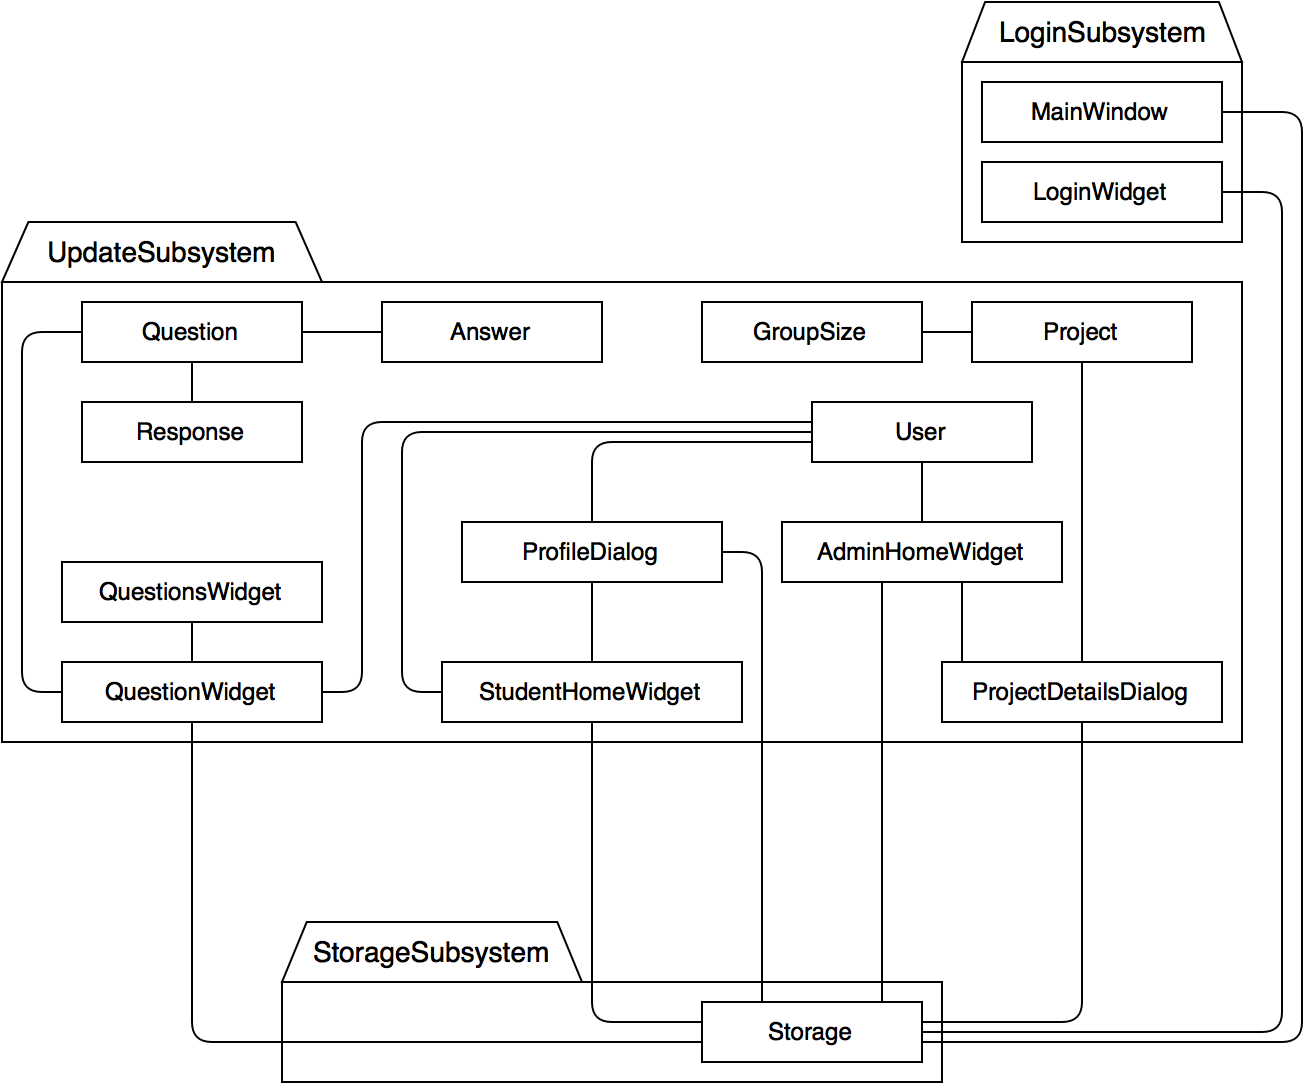
\includegraphics[scale=0.35]{imgs/d3/prototype/class-diagram.png}
	\caption{Subsystem Decomposition (Prototype)}
	\figurelabel{proto-decomp}
\end{figure}

\newpage{}
The following table, \tableref{proto-subsystems}, pulls the three subsystems mentioned above and provides a detailed description and unique identifier for each.

\begin{table}[H]
	\caption{Subsystems (Prototype)} \tablelabel{proto-subsystems}
    \begin{tabu} to \linewidth {l >{\it}l X}
        \tableheader{}ID & Name & Description \\
        \sdlabel{proto-storage}\sdref{proto-storage} & StorageSubsystem & The StorageSubsystem is in charge of retrieving information from the persistent storage to supply to the LoginSubsystem and the UpdateSubsystem. It also handles the updating of information to the persistent storage from the other subsystems.\\
        \sdlabel{proto-login}\sdref{proto-login} & LoginSubsystem & The LoginSubsystem is in charge of displaying the interface for the login and main window. It also verifies that the ID entered is valid through the StorageSubsystem. \\
        \sdlabel{proto-update}\sdref{proto-update} & UpdateSubsystem & The UpdateSubsystem encompasses all the classes that handle updating information in the persistent storage.\\
    \end{tabu}
\end{table}

\subsubsection{Subsystem Dependency Analysis}

The figure below, \figureref{proto-component}, illustrates the dependencies that exist between our three subsystems. In this prototype, we can see that both the UpdateSubsystem and the LoginSubsystem are dependent on the StorageSubsystem. While this component diagram clearly shows that our prototype does indeed follow the Repository architectural style, a style in which a StorageSubsystem has several subsystems that are dependent on it, the breakdown into subsystems still requires much tweaking. As we mentioned earlier, our subsystem division left much to be desired with regards to coupling.

\begin{figure}[H]
	\centering{}
	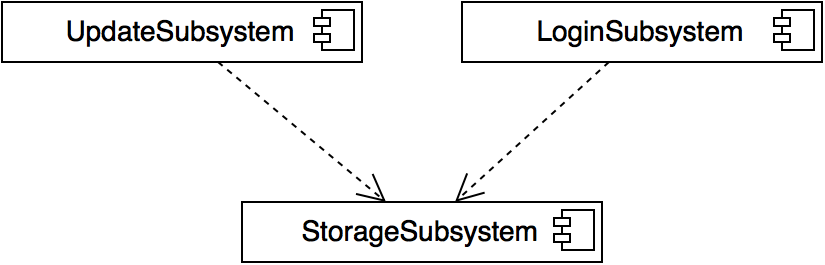
\includegraphics[scale=0.35]{imgs/d3/prototype/component-diagram.png}
	\caption{Component Diagram (Prototype)}
	\figurelabel{proto-component}
\end{figure}

\subsection{System Decomposition}
\subsubsection{Subsystem Decomposition}

The following figure, \figureref{subsys-decomp}, showcases our updated system decompostion. Note here that we have increased the amount of subsystems from three to six, as well as rearranged the classes inside each. Our subsystems now include: ProfileSubsystem, LoginSubsystem, UserSubsystem, PPIDSubsystem, ProjectSubsystem, and, of course, StorageSubsystem. This updated desion features extremely low coupling matched with a high degree of cohesion, which are ideal in a system.

\begin{figure}[H]
	\centering{}
	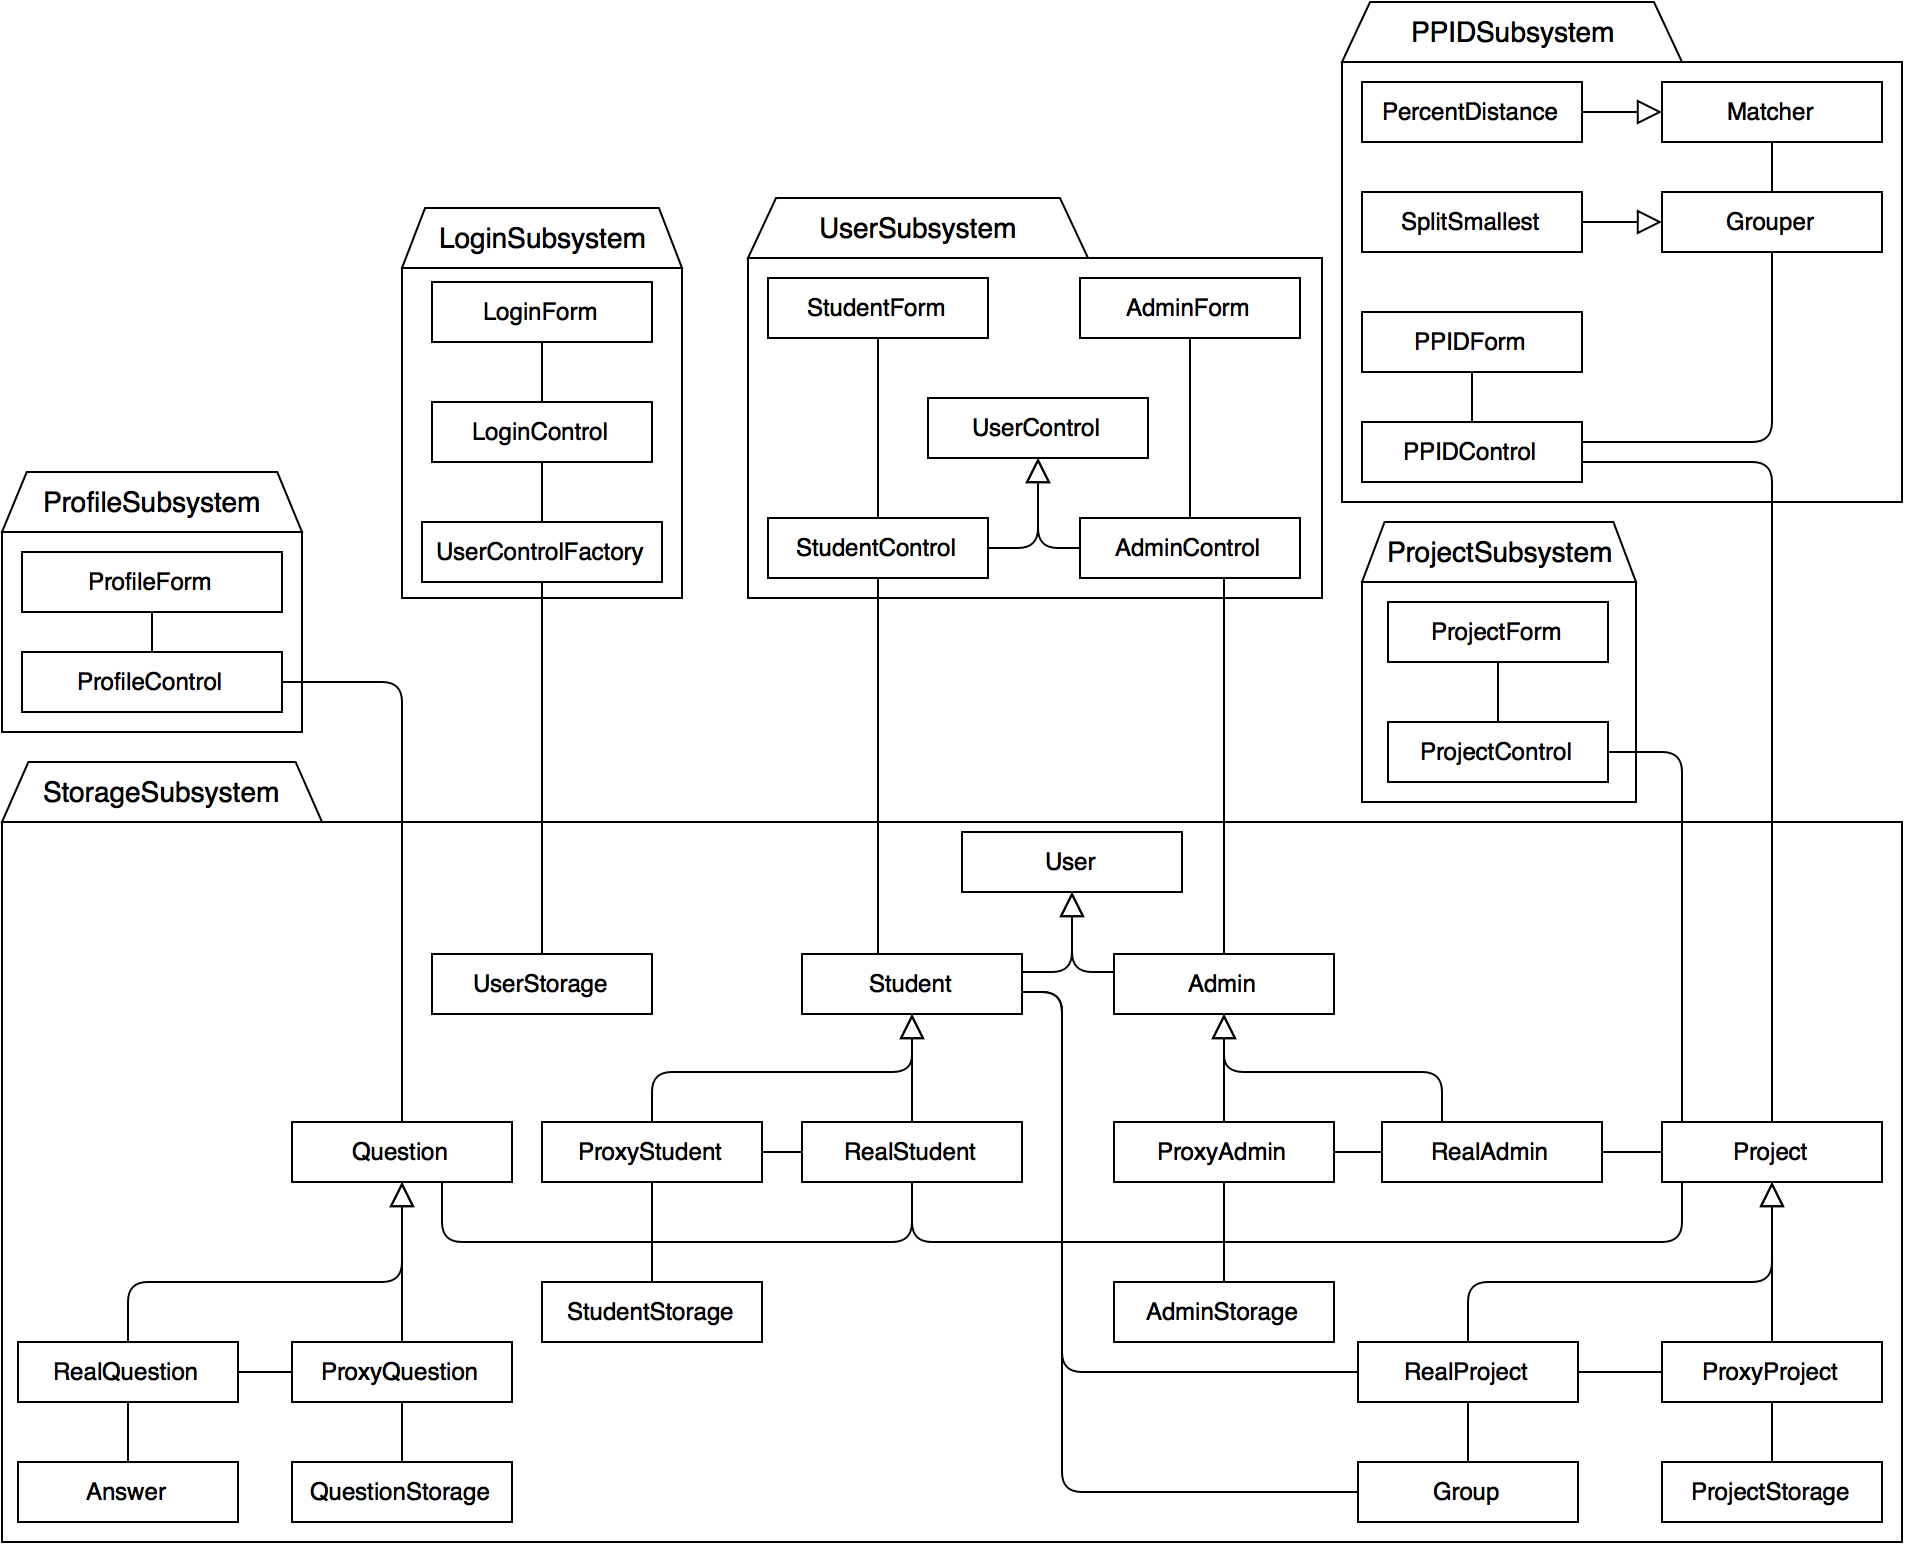
\includegraphics[scale=0.25]{imgs/d3/decomp/repository.png}
	\caption{Subsystem Decomposition}
	\figurelabel{subsys-decomp}
\end{figure}

The table below, \tableref{subsystems}, pulls the six subsystems mentioned above and provides a detailed description and unique identifier for each.

\begin{table}[H]
	\caption{Subsystems} \tablelabel{subsystems}
    \begin{tabu} to \linewidth {l >{\it}l X}
        \tableheader{}ID & Name & Description \\
        \sdlabel{login}\sdref{login} & LoginSubsystem & The LoginSubsystem handles the logging in aspect of our system. It checks with the StorageSubsystem to see if the ID entered exists before sending the user to the appropriate class in the UserSubsystem.\\
        \sdlabel{user}\sdref{user} & UserSubsystem & The UserSubsystem handles the main menu for each of the types of users (Student \& Admin). They present various options to the user and sends them to the appropriate subsystem afterwards.\\
    \end{tabu}
\end{table}

\begin{center}
\begin{tabu} to \linewidth {l >{\it}l X}
        \tableheader{}ID & Name & Description \\
	\sdlabel{profile}\sdref{profile} & ProfileSubsystem & The ProfileSubsystem handles the viewing and modifying of a Student's profile.\\
        \sdlabel{ppid}\sdref{ppid} & PPIDSubsystem & The PPIDSubsystem handles the running of the PPID algorithm.\\
        \sdlabel{project}\sdref{project} & ProjectSubsystem & The ProjectSubsystem handles the creation, deletion, and modification of Projects.\\
        \sdlabel{storage}\sdref{storage} & StorageSubsystem & The StorageSubsystem handles all the retrieval and writing from/to the persistent storage.\\
\end{tabu}
\end{center}

\subsubsection{Subsystem Dependency Analysis}

The figure below, \figureref{component}, illustrates the dependencies that exist between our six subsystems. In this updated system, we can see that all the subsystems other than the StorageSubsystem are dependent on the StorageSubsystem. This layout of subsystems showcases the Repository architectural style, wherein all subsystems are dependent on a repository subsystem (or storage subsystem). 

\begin{figure}[H]
	\centering{}
	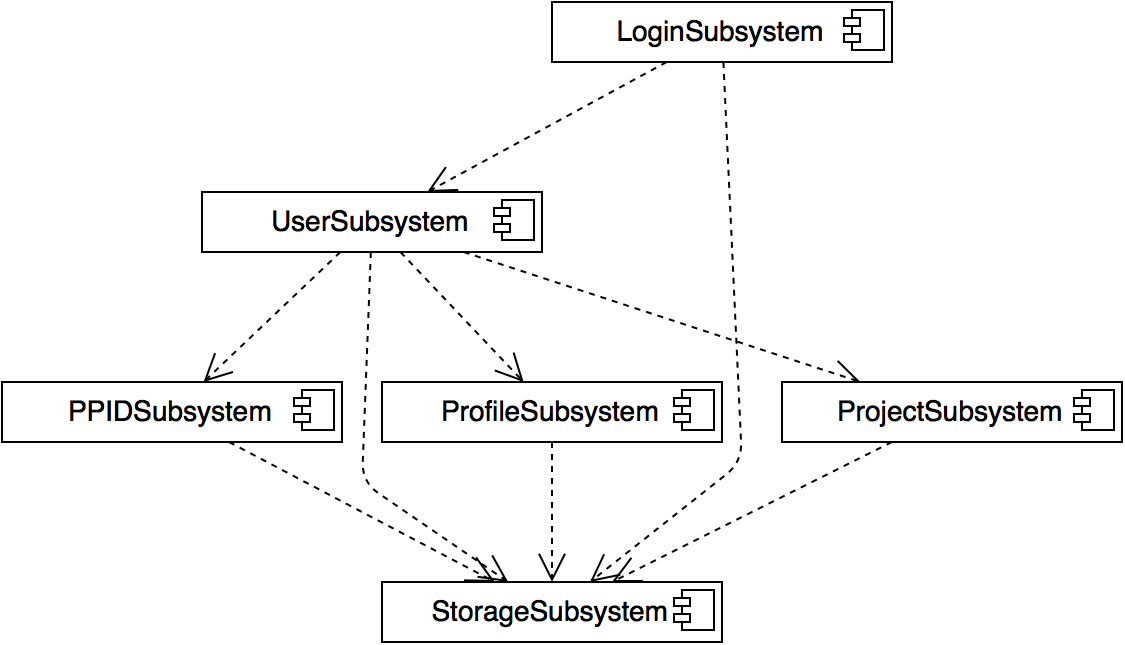
\includegraphics[scale=0.27]{imgs/d3/decomp/component-diagram.png}
	\caption{Component Diagram}
	\figurelabel{component}
\end{figure}

\subsection{Design Evolution}

This section will explain the various design decisions we made for the new, updated system. The goal of this new system is to maximize the amount of cohesion in our subsystems while minimizing the degree of coupling. While some of our decisions did involve architectural styles and design patterns, they will only be briefly discussed in this section. The following section will provide a more detailed explanation of why we decided on a particular pattern or style over another.

\subsubsection{Design Decisions}

Our prototype design, shown in \figureref{proto-decomp}, can be defined as the Repository architectural style. All the major necessary components are indeed present to earn that title. That said, however, because our implementation did not consider attempting to maximize cohesion and minimize coupling, we ended up with an extremely high degree of coupling between our subsystems. Specifically, due to the nature of the widgets that we used, there was no distinction between the view and the logic. It ended up, actually, that our widgets did mostly everything. Plus, every widget was highly dependent on the Storage. While normally this might seem normal, our subsystems were organized such that our widgets were not part of the repository layer, thus resulting the high coupling we mentioned earlier. To fix this problem, we have decided to reorganize our widgets so that they are dependent on entity type objects. We also decomposed our enormous storage object into several smaller, more specific storage objects. This has the added benefit of keeping only the related operations together, which in turn increases our degree of cohesion in our subsystem. By introducing more focused subsystems along with carefully used design patterns, like the proxy design pattern, we have limited the amount of inter-subsystem dependencies.

\section{Design Strategies}

Similar to the previous section, this section is also divided into three major parts: architectural style, persistent data management, and design patterns. In the first part, we will describe our chosen architectural style and explain the benefits to using this particular style with regards to our system. We will also include UML deployment diagrams as a visual representation of the architecture of our software. Following this part, we will discuss our design choices with regards to our persistent data management. We will also be covering some particular cases here, such as duplicate records. Finally, we will discuss our chosen design patterns and why they are appropriate given our decisions from the other parts in this section.

\subsection{Hardware/Software Mapping}
\subsubsection{Overview}

This section includes three separate parts: architectural styles, persistent data management, and design patterns. The first subsection will delve into the particular nuances of several architectural styles that we considered for our system and whether or not we decided to go with them. Included for each style will be some justification as to whether or not we believed them to be suitable. The following subsection dives into the particularities and details of our chosen persistent storage system. This subsection will include define all the tables that we use in our storage as well as the relationships existing between them. Finally, the last subsection will provide a detailed discussion of several different design patterns. Included in this discussion will be our reasoning as to whether or not we believe them to be appropriate for our system design. 

\subsubsection{Architectural Style}

Our system revolves heavily upon a central storage, or repository. Other than the repository, we make use of several subsystems. Simply with this in mind, we can instantly rule out the {\it pipe and filter} architectural style - while we do indeed have subsystems (filters) that associate with each other (pipes), our subsystems are fairly dependent on one another. Furthermore, our subsystems are responsible for more than simply processing a set of inputs to get a set of outputs. 

We can also rule out the four-tier architectural style right away - our system is entirely local, thus a separate client and server layer are unnecessary. We use a login-type system, and the UI is common to any user that logs in. The only difference would be that the displayed information changes, as well as some usability. That said, this type of functionality would best fit as multiple partitions within a layer. As a result, the difference in the student and admin users should be as sister partitions within the same layer.

\subsubsection*{Three-Tier Architecture}

Three-tier architecture involves dividing the system into three layers - the interface layer, the logic layer, and the storage layer. While it is more than possible, and, indeed, even appealing to consider such a decomposition, we decided not to go with this style. Unfortunately, this style, while having fairly high cohesion, has equally high coupling. For these reasons, we have decided to discard this architectural style. The figure below, \figureref{three-tier}, shows an updated version of our prototype model designed in the Three-Tier architectural style. With this visual, it is easier to see that the amount of dependencies that span across subsystems is enormous.

\begin{figure}[H]
	\centering{}
	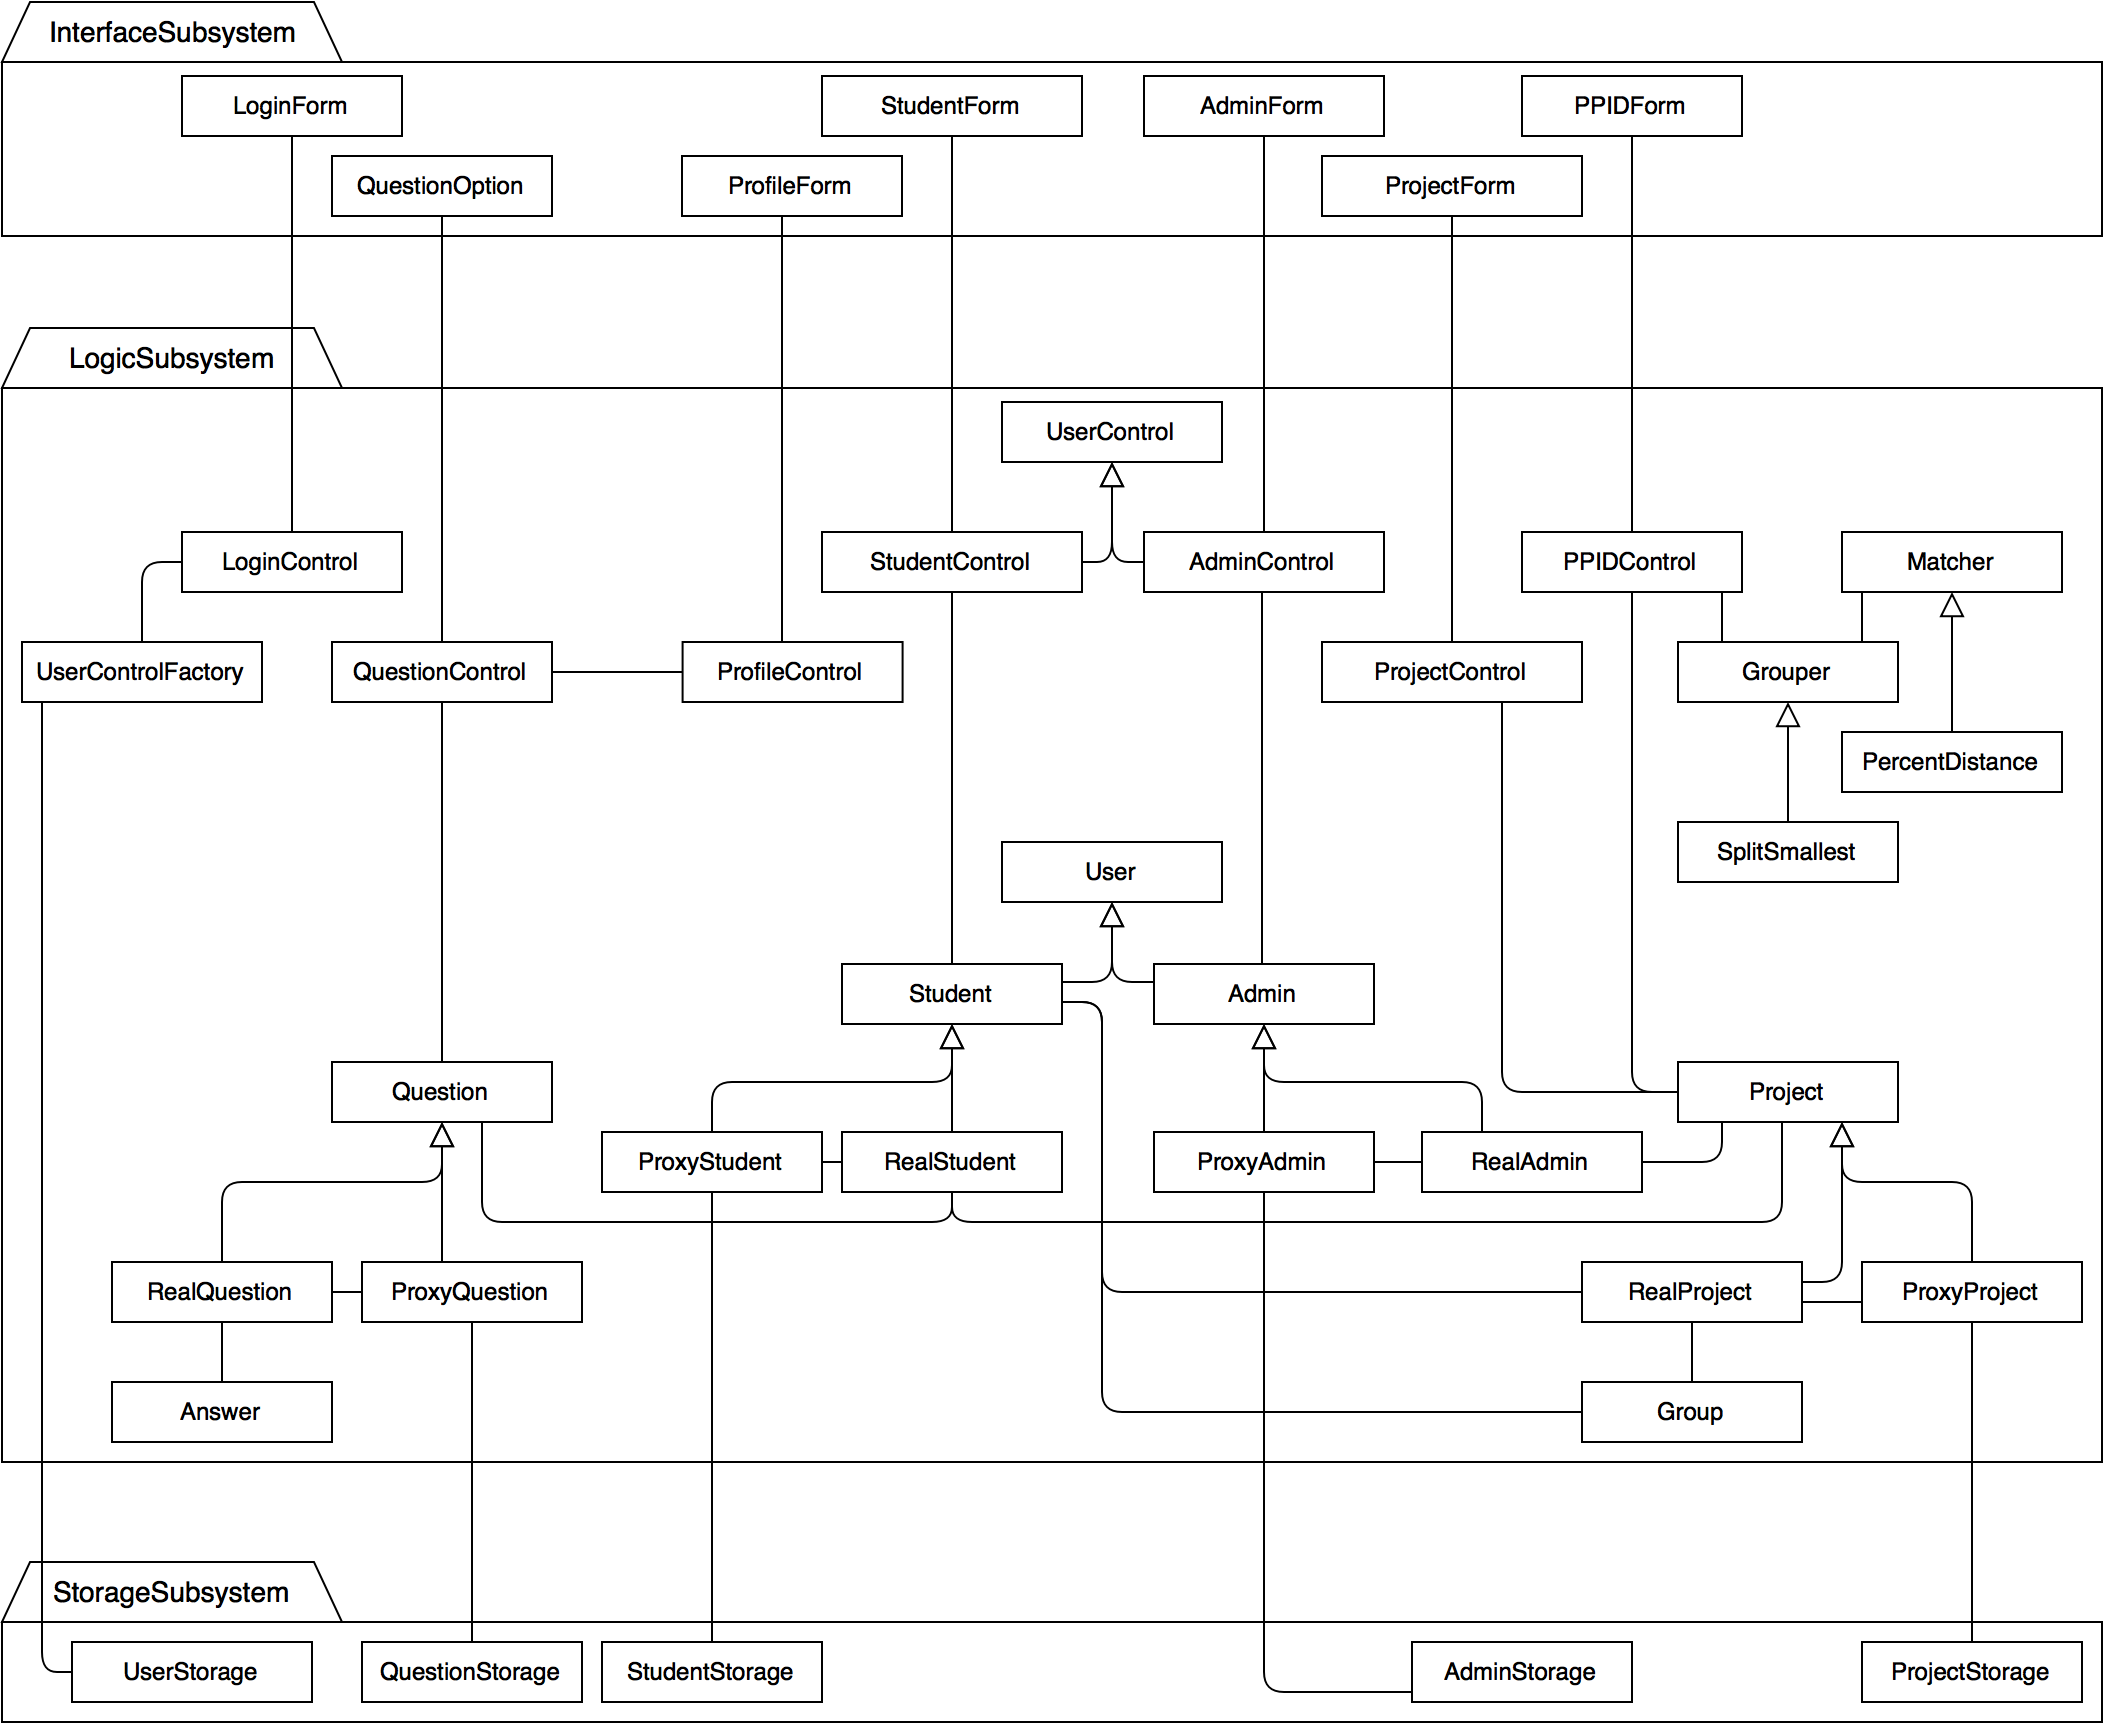
\includegraphics[scale=0.22]{imgs/d3/decomp/three-tier.png}
	\caption{Three-Tier Subsystem Decomposition}
	\figurelabel{three-tier}
\end{figure}
\subsubsection*{Model-View-Controller Architecture}

The Model-View-Controller architectural style involves three basic layers - the model layer, the view layer, and the controller layer. Unfortunately, due to the way our system is, if we were to employ this architectural style, we would have extremely high coupling (because the view and controller objects are in different subsystems). While the level of cohesion is still fairly high, none of this is lost if we were to switch over to say the Repository architectural style. In essence, using this architectural style brings no benefits to the table, but offers heavy drawbacks. For these reasons, we have decided not to use this architectural style.

\subsubsection*{Repository Architecture}

The Repository architectural style involves an absolutely necessary storage layer, followed by many subsystems one that depend on the storage layer. This is the architectural style that we employed, albeit poorly, in our prototype system - we have decided that the best course of action, after revamping our subsystem decomposition, is this architectural style: we can achieve extremely high cohesion along with minimal coupling. This means that there are very few interdependencies between different subsystems. The figure below, \figureref{repository}, provides a visual representation of the what the system would look like if properly implementing the repository architectural style.

\begin{figure}[H]
	\centering{}
	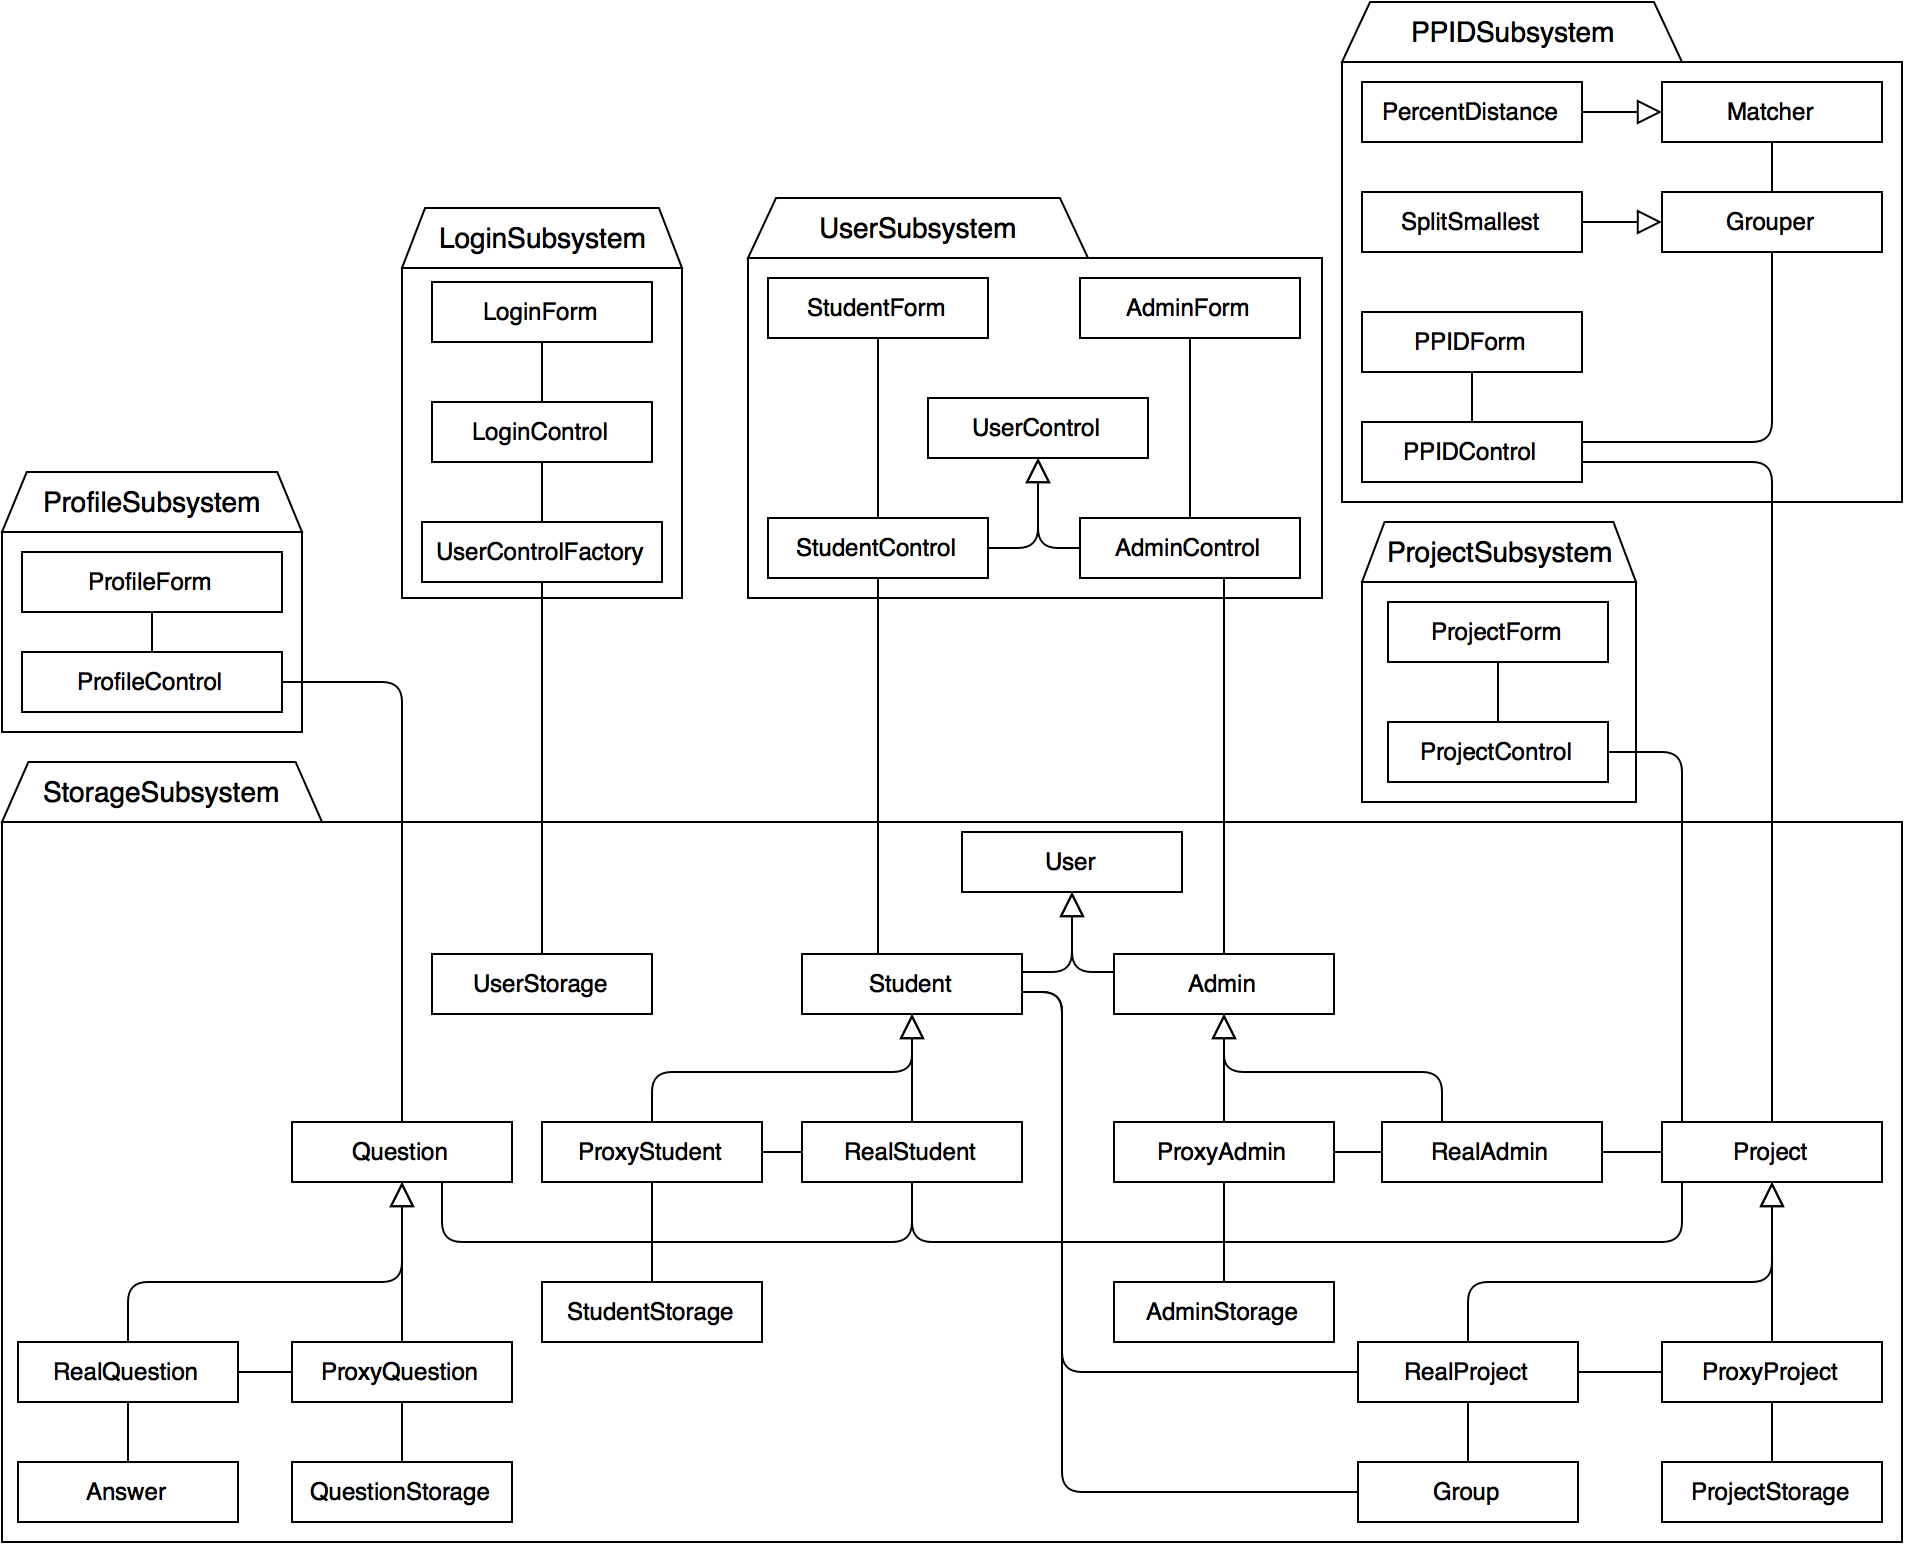
\includegraphics[scale=0.25]{imgs/d3/decomp/repository.png}
	\caption{Repository Subsystem Decomposition}
	\figurelabel{repository}
\end{figure}

\newpage{}
\subsubsection{Node Assignment}

The following figure, \figureref{deployment}, represents the node assignment of the entire system. Note that we have simply included the entire system to be assigned to the :UbuntuHost device - all the other subsystems are components of the System.

\begin{figure}[H]
	\centering{}
	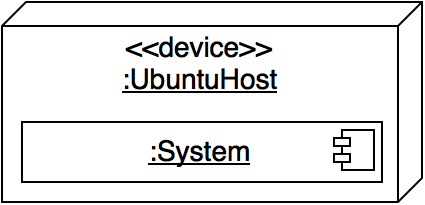
\includegraphics[scale=0.45]{imgs/d3/decomp/deployment-diagram.png}
	\caption{Deployment Diagram}
	\figurelabel{deployment}
\end{figure}

\subsubsection{Runtime Components}

The following figure, \figureref{runtime}, serves to provide a UML-based visual of the subsystems wherein the subsystem are grouped together into runtime components. 


\begin{figure}[H]
	\centering{}
	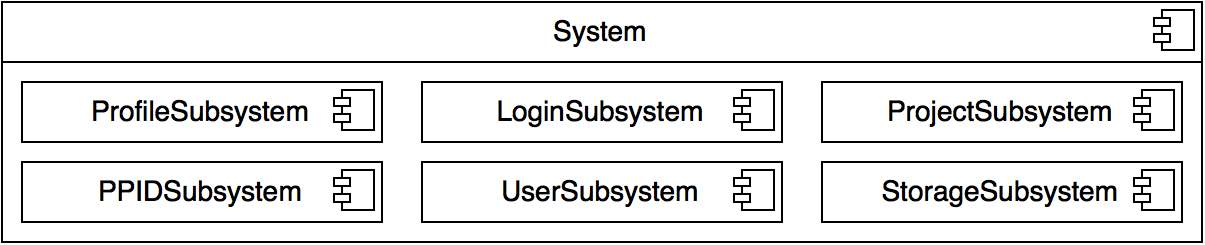
\includegraphics[scale=0.35]{imgs/d3/decomp/runtime-component-diagram.png}
	\caption{Runtime Component Diagram}
	\figurelabel{runtime}
\end{figure}

\subsection{Persistent Data Management}
\subsubsection{Overview}

To store the data for our system, a relational database is being used. Our relational database is built in the SQLite architecture. Multiple tables are used to store related information together, such as the \textit{students} table. The below figure, \figureref{db-schema}, shows a detailed schematics of the relations existing between all the tables that we have in our relational database. Note that each column in each table is listed alongside their data types.

\begin{figure}[H]
	\centering{}
	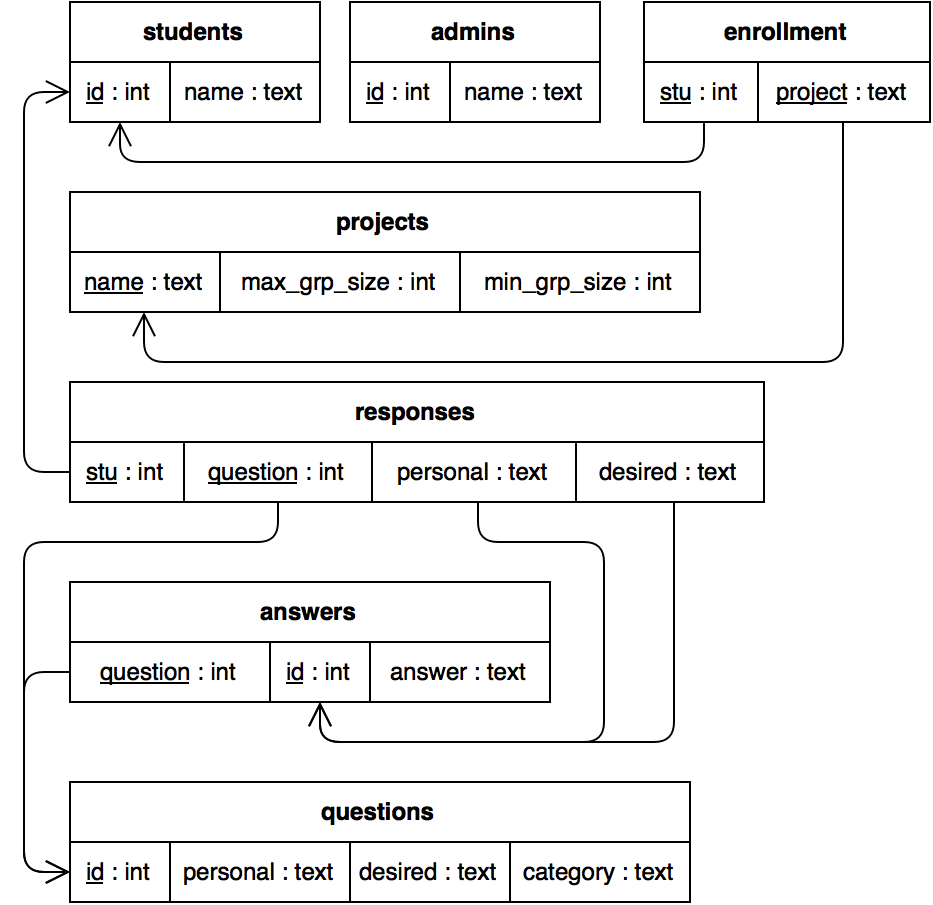
\includegraphics[scale=0.35]{imgs/d3/db/database-schema-diagram.png}
	\caption{Database Schema}
	\figurelabel{db-schema}
\end{figure}

While figures are great for visualization, what do these tables actually represent? The following table, \tableref{db-table}, describes what each table in our relational database represents. Each of these tables are assigned a unique identifier to allow for maximum traceability.

\begin{table}[H]
	\caption{Database Tables} \tablelabel{db-table}
	\begin{tabu} to \textwidth {l >{\it}l X}
		\tableheader{}ID & Name & Description \\
		\dtlabel{students}\dtref{students}     & students   & Stores the \textit{Student} (\cdref{student}) entity object. \\
		\dtlabel{admins}\dtref{admins}         & admins     & Stores the \textit{Admin} (\cdref{admin}) entity object. \\
		\dtlabel{projects}\dtref{projects}     & projects   & Stores the \textit{Project} (\cdref{project}) entity object. \\
		\dtlabel{enrollment}\dtref{enrollment} & enrollment & Stores the association between the \textit{Student} (\cdref{student}) 
		                                                      and \textit{Project} (\cdref{project}) entity objects, which is refers 
		                                                      to a student's enrollment into a project. \\
		\dtlabel{questions}\dtref{questions}   & questions  & Stores the \textit{Question} (\cdref{question}) entity object. \\
		\dtlabel{answers}\dtref{answers}       & answers    & Stores the \textit{Answer} (\cdref{answer}) entity object. \\
		\dtlabel{responses}\dtref{responses}   & responses  & Stores the association between the \textit{Student} (\cdref{student}) 
		                                                      and \textit{Question} (\cdref{question}) entity objects, which refers to      
		                                                      what answer a student has selected for a question. \\
	\end{tabu}
\end{table}

\subsubsection{Breakdown \& Reasoning}

\subsubsection*{Students Table (\dtref{students})}
To ensure that ID of a \textit{Student} (\cdref{student}) is unique, the \textit{id} column is set as the primary key. This guarantees that no two IDs can be equal.

There isn't a constraint put on the \textit{name} column to allow for \textit{Students} with the same name to be entered into the database. The following table, \tableref{students-table}, gives a more detailed breakdown and description of each of the columns of the \textit{students} table.

\begin{table}[H]
	\caption{Students Table (\dtref{students})} \tablelabel{students-table}
	\begin{tabu} to \textwidth {l l l X}
		\tableheader{}Column & Type & Constraint & Description \\
		id   & Integer & Primary Key & The unique ID given to the Student. \\
		name & Text    &             & The name of the Student. \\
	\end{tabu}
\end{table}

\subsubsection*{Administrator Table (\dtref{admins})}
To ensure that ID of a \textit{Admin} (\cdref{admin}) is unique, the \textit{id} column is set as the primary key. This guarantees that no two IDs can be equal. As well, by having the \textit{id} column as the primary key, the speed of looking up a \textit{Admin} by their ID is increased.

There isn't a constraint put on the \textit{name} column to allow for \textit{Admins} with the same name to be entered into the database. The following table, \tableref{admins-table}, gives a more detailed breakdown and description of each of the columns of the \textit{admins} table.

\begin{table}[H]
	\caption{Admins Table (\dtref{admins})} \tablelabel{admins-table}
	\begin{tabu} to \textwidth {l l l X}
		\tableheader{}Column & Type & Constraint & Description \\
		id   & Integer & Primary Key & The unique ID given to the Admin. \\
		name & Text    &             & The name of the Admin. \\
	\end{tabu}
\end{table}

\subsubsection*{Projects Table (\dtref{projects})}
Each \textit{Project} object (\cdref{project}) has a unique ID to uniquely identify it when querying or for referencing it in other tables. This ID is stored in the \textit{id} column, which is the primary key for the table. \textit{id} is used as the primary key oppose to the \textit{name} column, even though \textit{name} is always going to be unique as well, due to the fact the column is being referenced in other tables. If a \textit{Project's} name is changed, not only must it be changed in the \textit{name} column, but in every table it is referenced as well. That operation can be time consuming and, most importantly, may lead to errors causing the data in the database to be incorrect. By using an ID that will never change, then the name of the \textit{Project} can change without fear of corrupting data.

The following table, \tableref{projects-table}, gives a more detailed breakdown and description of each of the columns of the \textit{projects} table.

\begin{table}[H]
	\caption{Projects Table (\dtref{projects})} \tablelabel{projects-table}
	\begin{tabu} to \textwidth {l l X X[3]}
		\tableheader{}Column & Type & Constraint & Description \\
		id             & Integer & Primary Key      & The unique ID given to a Project. \\
		name           & Text    & Unique,\newline 
		                           Case Insensitive & The unique name given to a Project. \\
		max\_grp\_size & Integer &                  & The maximum group size of a Project. \\
		min\_grp\_size & Integer &                  & The minimum group size of a Project. \\
	\end{tabu}
\end{table}

\subsubsection*{Enrollment Table (\dtref{enrollment})}
Its important that each student can only enroll in each project once. To accomplish this, as shown in table \tableref{enrollment-table}, the \textit{enrollment} table has two columns: \textit{stu}, to reference the \textit{id} column from \textit{students} table (\dtref{students}), and \textit{project}, to reference \textit{id} from the \textit{projects} (\dtref{projects}). The primary key is then made up of both columns to ensure that only one instance of a \textit{students} entry and \textit{projects} entry combination exists at one time.

\begin{table}[H]
	\caption{Enrollment Table (\dtref{enrollment})} \tablelabel{enrollment-table}
	\begin{tabu} to \textwidth {l l X X[4]}
		\tableheader{}Column & Type & Constraint & Description \\
		stu     & Integer & Primary Key,\newline
		                    Foreign Key          & References \textit{id} of the \textit{students} table (\dtref{students}). \\
		project & Integer & Primary Key,\newline
		                    Foreign Key          & References \textit{id} of the \textit{projects} table (\dtref{projects}). \\
	\end{tabu}
\end{table}

\subsubsection*{Questions Table (\dtref{questions})}
The column \textit{id} in the \textit{questions} table stores a unique ID for a given question and is set as the primary key for the table. This allows for uniquely identifying a question which is very important for faster look up speeds and for referencing in other tables, which is required in this database.

The following table, \tableref{questions-table}, gives a more detailed breakdown and description of each of the columns of the \textit{questions} table.

\begin{table}[H]
	\caption{Questions Table (\dtref{questions})} \tablelabel{questions-table}
	\begin{tabu} to \textwidth {l l l X}
		\tableheader{}Column & Type & Constraint & Description \\
		id       & Integer & Primary Key & The unique identifier given to a Question. \\
		personal & Text    &             & Asks the Student to describe their self. \\
		desired  & Text    &             & Asks the Student to described their desired partner. \\
		category & Text    &             & The qualification category the Question belongs. \\
	\end{tabu}
\end{table}

\subsubsection*{Answers Table (\dtref{answers})}
In the system, an \textit{Answer} appears only once in a \textit{Question}, therefore the database should model that. To accomplish this, the primary key of the \textit{answers} table is made up of two columns: \textit{question}, which references the \textit{id} from the \textit{questions} table (\dtref{questions}), and \textit{id}, which is a unique ID for each \textit{Answer}. By having both columns as the primary key, this ensures that only one combination of \textit{question} and \textit{id} exist. That means a \textit{Question} can only have one occurrence of an \textit{Answer}.

The following table, \tableref{answers-table}, gives a more detailed breakdown and description of each of the columns of the \textit{answers} table.

\begin{table}[H]
	\caption{Answers Table (\dtref{answers})} \tablelabel{answers-table}
	\begin{tabu} to \textwidth {l l X X[4]}
		\tableheader{}Column & Type & Constraint & Description \\
		question & Integer & Primary Key,\newline
		                     Foreign Key          & The Question the answer belongs to. References \textit{id} of the 
		                                            \textit{questions} table. \\
		id       & Integer & Primary Key          & The unique ID given to the Answer. \\
		answer   & Text    &                      & The answer of a Question. \\
	\end{tabu}
\end{table}

\subsubsection*{Responses Table (\dtref{responses})}
A \textit{Student} is going to have one, and only one, response for every \textit{Question}. In that response, a \textit{Student} has a desired and personal value. To model this relationship, as shown in table \tableref{responses-table}, \textit{responses} table has a primary key made up of two columns: \textit{stu}, which references \textit{id} from the \textit{students} table (\dtref{students}), and \textit{question}, which references \textit{id} from the \textit{questions} table (\dtref{questions}). This ensures that a \textit{Student} can have only one response for a given \textit{Question}.

To deal with the desired and personal values, \textit{responses} has two other columns: \textit{personal}, and \textit{desired}. Both of these columns reference \textit{id} from the \textit{answers} table (\dtref{answers}).

\begin{table}[H]
	\caption{Responses Table (\dtref{responses})} \tablelabel{responses-table}
	\begin{tabu} to \textwidth {l l X X[4]}
		\tableheader{}Column & Type & Constraint & Description \\
		stu      & Integer & Primary Key,\newline
		                     Foreign Key          & Identifies the associated Student with the response. References \textit{id} of the 
		                                            \textit{students} table. \\
		question & Integer & Primary Key,\newline
		                     Foreign Key          & Identifies which Question the response belongs to. References \textit{question}
		                                            of the \textit{answers} table. \\
		personal & Integer & Foreign Key          & Identifies a Student's selection for their personal attribute for the given
		                                            given question. References \textit{id} of the \textit{answers} table. \\
		desired  & Integer & Foreign Key          & Identifies a Student's selection for their desired attribute for the given
		                                            given question. References \textit{id} of the \textit{answers} table. \\
	\end{tabu}
\end{table}

\subsection{Design Patterns}
\subsubsection{Overview}
While organizing code with an eye to the larger picture - architectural styles - is vitally important, the smaller scale design patterns fall not far behind. Design patterns are largely independent of the architectural style insofar as nearly all design patterns can be implemented in any of the architectural patterns. They usually are used to minimize coupling across layers or to maximize cohesion across sister subsystems (partitions). This section will go over several different design patterns and explain either why we decide to use them or why we forgo their implementation. There are three main categories of design patterns that we will include in this breakdown: creational patterns, structural patterns, and behavioural patterns.
\subsubsection{Creational Patterns}
The design patterns in this section affect how objects get created. There will be one pattern in this section that we will be considering for our system: the factory method design pattern. 

\subsubsection*{Factory Method}
We have decided to implement this design pattern in our system. The idea for this pattern is define a specialized interface for object creation that lets subclasses make the decision as to which particular class to instantiate. This pattern is apparent a user attempts to login - we do not know initially what type of user is logging in. In this scenario, we let UserStorage class tell us what type of user it is and then the UserControlFactory class will instantiate it. Another way of seeing this pattern is to imagine the UserControlFactory as a Template method - there is a placeholder of sorts that subclasses will specify. The figure below, \figureref{factmethod-example}, provides a small, simple UML-based visual of how the Factory Method pattern is set up. Note that the factory class has a method makeObject(). This method asks the subclass to know what kind of object it needs to be making.

\begin{figure}[H]
	\centering{}
	\includegraphics[scale=0.55]{imgs/d3/sample-factmethod.png}
	\caption{Example of the Factory Method Design Pattern}
	\figurelabel{factmethod-example}
\end{figure}

\subsubsection{Structural Patterns}
The design patterns in this section affect the relationships between objects. Specifically, they aim to simplify their implementation. There are three patterns that we considered implementing in our system: the adapter design pattern, the facade design pattern, and the proxy design pattern.

\subsubsection*{Adapter}
This design pattern is ill suited to our particular system since we will be developing the entirety of our system. Since we will not need to write code that adapts between newer and older code, this pattern would be counter-intuitive. The way that the adapter pattern works is that it converts an existing interface of a class into an typically older, or `legacy', interface that the client is more familiar with. As mentioned earlier, our system uses no old components, so this pattern will not fit in. The below figure, \figureref{adapter-example}, provides a small UML-based visual of how the Adapter Pattern is set up. Note here that the Interface represents an old interface that the NewObject must `adapt' to.

\begin{figure}[H]
	\centering{}
	\includegraphics[scale=0.55]{imgs/d3/sample-adapter.png}
	\caption{Example of the Adapter Design Pattern}
	\figurelabel{adapter-example}
\end{figure}

\subsubsection*{Facade}
We heavily considered using this design pattern. Initially, it seemed like our subsystems were fairly complex, but, after reorganizing things, we managed to simplify everything greatly. With that in mind, the facade pattern no longer seemed appealing. The facade pattern is specifically designed to provide a simple interface to a complex subsystem. Since our subsystems ended up rather simplisitic, using the facade pattern would simply be an additional level of complexity, which is extremely counter-intuitive to the purpose of using this design pattern. The figure below, \figureref{facade-example}, provides a small UML-based visual of how the Facade Pattern is set up. Note here that the Facade is the class interacting with the Client - it provides a simplified interface and does the actual complicated work behind the scenes.

\begin{figure}[H]
	\centering{}
	\includegraphics[scale=0.45]{imgs/d3/sample-facade.png}
	\caption{Example of the Facade Design Pattern}
	\figurelabel{facade-example}
\end{figure}

\subsubsection*{Proxy}
We have chosen to implement this design pattern in our system. By encompassing several of our entity objects in a proxy design, we can implement a `lazy' load-type system in that the system will only load the information that we directly ask for - nothing extra. This has the enormous benefit of reducing the memory footprint. The time trade-off is comparably minimal, even negligible. The following figure, \figureref{proxy-example}, provides a small UML-based visual of how the Proxy Pattern is set up. The idea is that the ProxyObject acts as a kind of interface to the RealObject, wherein the rest of the system has no access to the RealObject.

\begin{figure}[H]
	\centering{}
	\includegraphics[scale=0.55]{imgs/d3/proxy-example.png}
	\caption{Example of the Proxy Design Pattern}
	\figurelabel{proxy-example}
\end{figure}

\subsubsection{Behavioural Patterns}
The design patterns in this section are concerned with communication patterns between different objects. Specifically, they aim to provide a regular, common communication pattern. There are two patterns that we are considering in this section: the observer design pattern and the strategy design pattern.

\subsubsection*{Observer}

This design pattern is at the heart of the Model-View-Controller architectural style. It involves a one-to-many dependency between multiple objects such that when the one object changes state, all the `observing' objects are notified and updated automatically. We heavily considered implementing this design pattern while we were still considering between using Model-View-Controller and using Repository Style. That said, the MVC style resulted in a high degree of coupling, so we decided to go with the more basic Repository Style. Because of the way that we set up our system now, there is no need for the Observer Pattern - objects pull their information directly from the persistent storage whenever there is a need to display. Because of this peculiarity, updating the UI objects that a change has been made would be useless. The following figure, \figureref{observer-example}, provides a small UML-based visual on how the Observer Pattern is set up.

\begin{figure}[H]
	\centering{}
	\includegraphics[scale=0.55]{imgs/d3/sample-observer.png}
	\caption{Example of the Observer Design Pattern}
	\figurelabel{observer-example}
\end{figure}

\subsubsection*{Strategy}

We have decided to implement this pattern in our system, though it may not seem obviously apparent as to why initially. While it is true that it currently serves little to no purpose, it acts as a future-proofing mechanism. It is entirely possible that at some point in time we may want to extend the functionality of our system to include the usage of multiple different sorting algorithms - perhaps one for each field. By incorporating the Strategy Pattern, we have given our system the tools to easily handle this change. This class has the huge benefit of minimizing coupling - other classes are coupled only to an abstraction, thus added more derived classes wouldn't change anything for them. The below figure, \figureref{strategy-example}, provides a small UML-based visual on how the Strategy Pattern is set up.

\begin{figure}[H]
	\centering{}
	\includegraphics[scale=0.45]{imgs/d3/sample-strategy.png}
	\caption{Example of the Strategy Design Pattern}
	\figurelabel{strategy-example}
\end{figure}

\section{Subsystem Services}
\subsection{Overview}

The following section will be divided into three major sections: services, operations, and component diagrams. The first section will cover all the different services that each subsystem offers, whereas the second section will concern itself with the various operations that each service requires and the corresponding classes that offer those operations. The final section will include component diagrams that showcase the services provided by each subsystem via the `ball-and-socket' notation.

\subsection{Services}

In this section, we give a list and description of each of the services that our subsystems offer. They will be divided into separate tables - one for each of our subsystems. To really emphasize our design, we will also include component diagrams for each subsystem in the UML `ball-and-socket' notation as visuals.

\newpage{}
\subsubsection{UserSubsystem (\sdref{user})}

\noindent{}
The following table, \tableref{user-services}, describes the service that is offered by the UserSubsystem (\sdref{user}).

\begin{table}[H]
	\caption{Services Offered by UserSubsystem (\sdref{user})} \tablelabel{user-services}
	\begin{tabu} to \textwidth {l >{\it}l X}
		\tableheader{}ID & Service & Description\\
		\sslabel{user-options}\ssref{user-options} & UserOptionsService & The UserOptionsService is a service that encompasses operations that, given a User type, starts up the appropriate User's main page.\\
	\end{tabu}
\end{table}

The figure below, \figureref{user-services}, shows the service offered by the UserSubsystem, UserOptionsService, along with the subsystem that uses that service (the LoginSubsystem) in the UML `ball-and-socket' notation.

\begin{figure}[H]
	\centering{}
	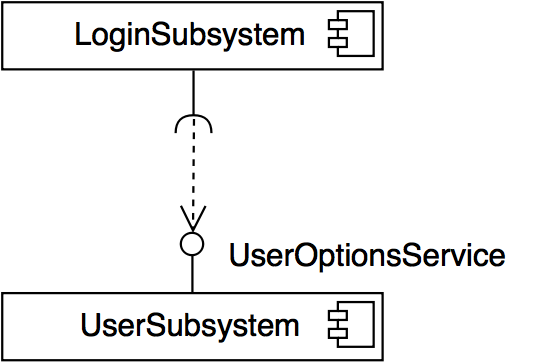
\includegraphics[scale=0.40]{imgs/d3/services/user-subsystem.png}
	\caption{Services Offered by UserSubsystem (\sdref{user})}
	\figurelabel{user-services}
\end{figure}

\subsubsection{ProfileSubsystem (\sdref{profile})}

\noindent{}
The following table, \tableref{profile-services}, describes the service that is offered by the ProfileSubsystem (\sdref{profile}).

\begin{table}[H]
	\caption{Services Offered by ProfileSubsystem (\sdref{profile})} \tablelabel{profile-services}
	\begin{tabu} to \textwidth {l >{\it}l X}
		\tableheader{}ID & Service & Description\\
		\sslabel{profile-options}\ssref{profile-options} & ProfileOptionsService & The ProfileOptionsService is a service that encompasses operations that allows a Student User to access and modify their Profiles.\\
	\end{tabu}
\end{table}

The figure below, \figureref{profile-services}, shows the service offered by the ProfileSubsystem, ProfileOptionsService, along with the subsystem that uses that service (the UserSubsystem) in the UML `ball-and-socket' notation.

\begin{figure}[H]
	\centering{}
	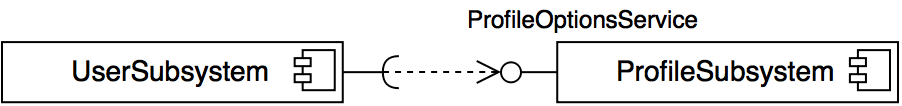
\includegraphics[scale=0.40]{imgs/d3/services/profile-subsystem.png}
	\caption{Services Offered by ProfileSubsystem (\sdref{profile})}
	\figurelabel{profile-services}
\end{figure}

\newpage{}
\subsubsection{ProjectSubsystem (\sdref{project})}

\noindent{}
The following table, \tableref{project-services}, describes the service that is offered by the ProjectSubsystem (\sdref{project}).

\begin{table}[H]
	\caption{Services Offered by ProjectSubsystem (\sdref{project})} \tablelabel{project-services}
	\begin{tabu} to \textwidth {l >{\it}l X}
		\tableheader{}ID & Service & Description\\
		\sslabel{project-options}\ssref{project-options} & ProjectOptionsService & The ProjectOptionsService is a service that encompasses operations that allows an Admin User to add, remove, or modify Projects.\\
	\end{tabu}
\end{table}

The figure below, \figureref{project-services}, shows the service offered by the ProjectSubsystem, ProjectOptionsService, along with the subsystem that uses that service (the UserSubsystem) in the UML `ball-and-socket' notation.

\begin{figure}[H]
	\centering{}
	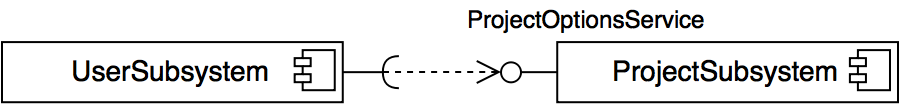
\includegraphics[scale=0.40]{imgs/d3/services/project-subsystem.png}
	\caption{Services Offered by ProjectSubsystem (\sdref{project})}
	\figurelabel{project-services}
\end{figure}

\subsubsection{PPIDSubsystem (\sdref{ppid})}

\noindent{}
The following table, \tableref{ppid-services}, describes the service that is offered by the PPIDSubsystem (\sdref{ppid}).

\begin{table}[H]
	\caption{Services Offered by PPIDSubsystem (\sdref{ppid})} \tablelabel{ppid-services}
	\begin{tabu} to \textwidth {l >{\it}l X}
		\tableheader{}ID & Service & Description\\
		\sslabel{ppid-options}\ssref{ppid-options} & PPIDOptionsService & The PPIDOptionsService is a service that encompasses operations that allow an Admin User to run the PPID algorithm on a selected Project.\\
	\end{tabu}
\end{table}

The figure below, \figureref{ppid-services}, shows the service offered by the PPIDSubsystem, PPIDOptionsService, along with the subsystem that uses that service (the UserSubsystem) in the UML `ball-and-socket' notation.

\begin{figure}[H]
	\centering{}
	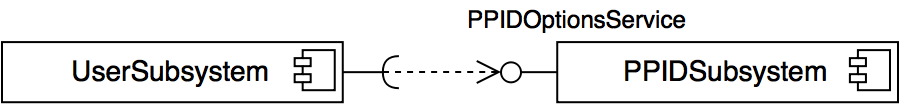
\includegraphics[scale=0.40]{imgs/d3/services/ppid-subsystem.png}
	\caption{Services Offered by PPIDSubsystem (\sdref{ppid})}
	\figurelabel{ppid-services}
\end{figure}

\newpage{}
\subsubsection{StorageSubsystem (\sdref{storage})}

The following table, \tableref{storage-services}, describes all the services that are offered by the StorageSubsystem (\sdref{storage}). 

\begin{table}[H]
	\caption{Services Offered by the StorageSubsystem (\sdref{storage})} \tablelabel{storage-services}
	\begin{tabu} to \textwidth {l >{\it}l X}
		\tableheader{}ID & Service & Description\\
		\sslabel{user}\ssref{user} & UserService & The UserService is a service that encompasses operations that allow subsystems to access values related to the User class.\\
		\sslabel{student}\ssref{student} & StudentService & The StudentService is a service that encompasses operations that allow subsystems to access values related to the Student objects.\\
		\sslabel{admin}\ssref{admin} & AdminService & The AdminService is a service that encompasses operations that allow subsystems to access values related to the Admin objects.\\
		\sslabel{project}\ssref{project} & ProjectService & The ProjectService is a service that encompasses operations that allow subsystems to access and modify values related to the Project objects.\\
		\sslabel{question}\ssref{question} & QuestionService & The QuestionsService is a service that encompasses operations that allow subsystems to access and modify values related to the Question objects.\\
	\end{tabu}
\end{table}

The figure below, \figureref{storage-services}, shows the services offered by the StorageSubsystem, UserService, StudentService, AdminService, ProjectService, and QuestionService, along with the subsystems that uses that service (the UserSubsystem, the LoginSubsystem, the ProjectSubsystem, the PPIDSubsystem, and the ProfileSubsystem) in the UML `ball-and-socket' notation.

\begin{figure}[H]
	\centering{}
	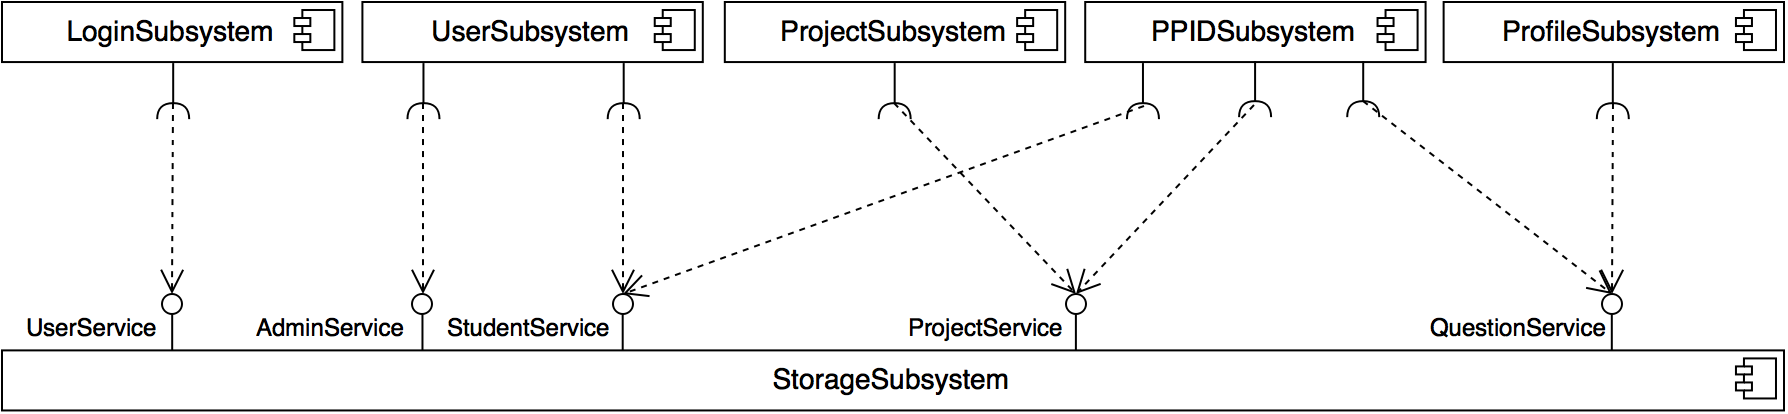
\includegraphics[scale=0.27]{imgs/d3/services/storage-subsystem.png}
	\caption{Services Offered by StorageSubsystem (\sdref{storage})}
	\figurelabel{storage-services}
\end{figure}

\subsection{Operations}

In this section, we focus on the Operations that each of the services described in the above section offer. For added traceability, we have also included the specific class that provides each of the operations, as well as a description of each.

\newpage{}
\subsubsection{UserOptionsService (\ssref{user-options})}

This section will include the class whose operation(s) are used in the UserOptionsService service (\ssref{user-options}). In the table below, \tableref{usercontrol-ops}, we feature an operation, start, provided by the UserControl Class (\cdref{user-ctrl}).

\begin{table}[H]
	\caption{UserControl Class (\cdref{user-ctrl}) Operations} \tablelabel{usercontrol-ops}
	\begin{tabu} to \textwidth {l >{\it}l X}
		\tableheader{}ID & Operation & Description \\
        \oplabel{user-ctrl-start}\opref{user-ctrl-start} & start() & Starts the UserControl (\cdref{user-ctrl}). \\
	\end{tabu}
\end{table}

\subsubsection{ProfileOptionsService (\ssref{profile-options})}

This section will include the class whose operation(s) are used in the ProfileOptionsService service (\ssref{profile-options}). In the table below, \tableref{profilecontrol-ops}, we feature an operation, start, provided by the ProfileControl Class (\cdref{profile-ctrl}).

\begin{table}[H]
	\caption{ProfileControl Class (\cdref{profile-ctrl}) Operations} \tablelabel{profilecontrol-ops}
	\begin{tabu} to \textwidth {l >{\it}l X}
		\tableheader{}ID & Operation & Description \\
        \oplabel{profile-ctrl-start}\opref{profile-ctrl-start} & start() & Starts the ProfileControl (\cdref{profile-ctrl}). \\
	\end{tabu}
\end{table}

\subsubsection{ProjectOptionsService (\ssref{project-options})}

This section will include the class whose operation(s) are used in the ProjectOptionsService service (\ssref{project-options}). In the table below, \tableref{projectcontrol-ops}, we feature an operation, start, provided by the ProjectControl Class (\cdref{project-ctrl}).

\begin{table}[H]
	\caption{ProjectControl Class (\cdref{project-ctrl}) Operations} \tablelabel{projectcontrol-ops}
	\begin{tabu} to \textwidth {l >{\it}l X}
		\tableheader{}ID & Operation & Description \\
        \oplabel{project-ctrl-start}\opref{project-ctrl-start} & start() & Starts the ProjectControl (\cdref{project-ctrl}). \\
	\end{tabu}
\end{table}

\subsubsection{PPIDOptionsService (\ssref{ppid-options})}

This section will include the class whose operation(s) are used in the PPIDOptionsService service (\ssref{ppid-options}). In the table below, \tableref{ppidcontrol-ops}, we feature an operation, start, provided by the PPIDControl Class (\cdref{ppid-ctrl}).

\begin{table}[H]
	\caption{PPIDControl Class (\cdref{ppid-ctrl}) Operations} \tablelabel{ppidcontrol-ops}
	\begin{tabu} to \textwidth {l >{\it}l X}
		\tableheader{}ID & Operation & Description \\
        \oplabel{ppid-ctrl-start}\opref{ppid-ctrl-start} & start() & Starts the PPIDControl (\cdref{ppid-ctrl}). \\
	\end{tabu}
\end{table}

\subsubsection{UserService (\ssref{user})}

This section will include the class whose operation(s) are used in the UserService service (\ssref{user}). In the table below, \tableref{userstorage-ops}, we feature two operations, getStudent and getAdmin, provided by the UserStorage Class (\cdref{user-storage}).

\begin{table}[H]
	\caption{UserStorage Class (\cdref{user-storage}) Operations} \tablelabel{userstorage-ops}
	\begin{tabu} to \textwidth {l >{\it}l X}
		\tableheader{}ID & Operation & Description \\
        \oplabel{user-storage-get-student}\opref{user-storage-get-student} & getStudent(in id : int) : Student & Gets the Student (\cdref{student}) with the specified ID from storage. \\
        \oplabel{user-storage-get-admin}\opref{user-storage-get-admin} & getAdmin(in id : int) : Admin & Gets the Admin (\cdref{admin}) with the specified ID from storage. \\
	\end{tabu}
\end{table}

\subsubsection{StudentService (\ssref{student})}

This section will include the class whose operation(s) are used in the StudentService service (\ssref{student}). In the table below, \tableref{student-ops}, we feature five operations, getQuestions, getEnrolledProjects, getAvailableProjects, joinProjects, and leaveProjects, provided by the Student Class (\cdref{student}).

\begin{table}[H]
	\caption{Student Class (\cdref{student}) Operations} \tablelabel{student-ops}
	\begin{tabu} to \textwidth {l >{\it}l X}
		\tableheader{}ID & Operation & Description \\
        \oplabel{user-get-questions}\opref{user-get-questions} & getQuestions() : List<Question> & Gets the Questions (\cdref{question}) containing the Student's (\cdref{student}) answers. \\
        \oplabel{user-get-enrolled-projects}\opref{user-get-enrolled-projects} & getEnrolledProjects() : List<Project> & Gets the Projects (\cdref{project}) in which the Student (\cdref{project}) is enrolled. \\
        \oplabel{user-get-available-projects}\opref{user-get-available-projects} & getAvailableProjects() : List<Project> & Gets the Projects (\cdref{project}) the Student (\cdref{project}) can join. \\
        \oplabel{user-join-project}\opref{user-join-project} & joinProject(in p : Project) & Places the Student (\cdref{student}) in the Project (\cdref{project}). \\
        \oplabel{user-leave-project}\opref{user-leave-project} & leaveProject(in p : Project) & Removes the Student (\cdref{student}) from the Project (\cdref{project}). \\
	\end{tabu}
\end{table}

\subsubsection{AdminService (\ssref{admin})}

This section will include the class whose operation(s) are used in the AdminService service (\ssref{admin}). In the table below, \tableref{admin-ops}, we feature three operations, getProjects, deleteProjects, and addProjects, provided by the Admin Class (\cdref{admin}).

\begin{table}[H]
	\caption{Admin Class (\cdref{admin}) Operations} \tablelabel{admin-ops}
	\begin{tabu} to \textwidth {l >{\it}l X}
		\tableheader{}ID & Operation & Description \\
        \oplabel{admin-get-projects}\opref{admin-get-projects} & getProjects() : List<Project> & Gets the Projects (\cdref{project}) all the projects. \\
        \oplabel{admin-delete-project}\opref{admin-delete-project} & deleteProject(in p : Project) & Deletes the Project (\cdref{project}). \\
        \oplabel{admin-add-project}\opref{admin-add-project} & addProject(in p : Project) & Adds the Project (\cdref{project}). \\
	\end{tabu}
\end{table}

\subsubsection{ProjectService (\ssref{project})}

This section will include the class whose operation(s) are used in the ProjectService service (\ssref{project}). In the table below, \tableref{project-ops}, we feature three operations, getStudents, getGroups, and setGroups, provided by the Project Class (\cdref{project}).

\begin{table}[H]
	\caption{Project Class (\cdref{project}) Operations} \tablelabel{project-ops}
	\begin{tabu} to \textwidth {l >{\it}l X}
		\tableheader{}ID & Operation & Description \\
        \oplabel{project-get-students}\opref{project-get-students} & getStudents() : List<Student> & Gets the enrolled Students (\cdref{student}). \\
        \oplabel{project-get-groups}\opref{project-get-groups} & getGroups() : List<Group> & Gets the Groups (\cdref{group}) of students created by the PPID. \\
        \oplabel{project-set-groups}\opref{project-set-groups} & setGroups(in g : List<Group>) & Sets the Groups (\cdref{group}). \\
	\end{tabu}
\end{table}

\subsubsection{QuestionService (\ssref{question})}

This section will include the class whose operation(s) are used in the QuestionService service (\ssref{question}). In the table below, \tableref{question-ops}, we feature five operations, getAnswers, getPersonal, getDesired, setPersonal, and setDesired, provided by the Question Class (\cdref{question}).

\begin{table}[H]
	\caption{Question Class (\cdref{question}) Operations} \tablelabel{question-ops}
	\begin{tabu} to \textwidth {l >{\it}l X}
		\tableheader{}ID & Operation & Description \\
        \oplabel{question-get-answers}\opref{question-get-answers} & getAnswers() : List<Answer> & Gets the possible Answers (\cdref{answer}). \\
        \oplabel{question-get-personal-answer}\opref{question-get-personal-answer} & getPersonalAnswer() : Answer & Gets the Answer (\cdref{answer}) to the personal question. \\
        \oplabel{question-get-desired-answer}\opref{question-get-desired-answer} & getDesiredAnswer() : Answer & Gets the Answer (\cdref{answer}) to the desired question. \\
        \oplabel{question-set-personal}\opref{question-set-personal} & setPersonal(in a : Answer) & Sets the Answer (\cdref{answer}) to the personal question. \\
        \oplabel{question-set-desired}\opref{question-set-desired} & setDesired(in a : Answer) & Sets the Answer (\cdref{answer}) to the desired question. \\
	\end{tabu}
\end{table}

\newpage{}
\section{Class Interfaces}

\subsection{Overview}
This section contains all the classes in our system, divided into subsections wherein each subsection represents a service. Along with a table containing a short, detailed description of each class, there will be a UML class diagram provided for each system to showcase the interactions between the classes.

%\subsection*{Section Contents}
%\vspace{0.5em}\hrule\vspace{0.5em}
%\startcontents[sections]
%\printcontents[sections]{}{1}{}
%\vspace{0.5em}\hrule\vspace{0.5em}

\subsection{UserOptionsService (\ssref{user-options})}

The following table, \tableref{user-option-classes}, describes each of the classes involved in the UserOptionsService service (\ssref{user-options}) as well as provide a unique identifier for each.
\begin{table}[H]
	\caption{UserOptionsService Classes (\ssref{user-options})} \tablelabel{user-option-classes}
	\begin{tabu} to \textwidth {l >{\it}l X}
	    \tableheader{}ID & Class Name & Description \\
	    \cdlabel{user-ctrl}\cdref{user-ctrl} & UserControl & The UserControl class contains only a single operation - start.\\
	    \cdlabel{student-ctrl}\cdref{student-ctrl} & StudentControl & The StudentControl class inherits from the UserControl class, and contains only the inherited start operation. This class controls the possible options that a Student can have.\\
	    \cdlabel{admin-ctrl}\cdref{admin-ctrl} & AdminControl & The AdminControl class inherits from the UserControl class, and contains only the inherited start operation. This class controls the possible options that an Admin can have. \\
	    \cdlabel{student-form}\cdref{student-form} & StudentForm & The StudentForm class is a UI-based class - the only operation that this class has is show. This class displays the information concerning the particular Student User that is currently logged in.\\
	    \cdlabel{admin-form}\cdref{admin-form} & AdminForm & The AdminForm class is a UI-based class - the only operation that this class has is show. This class displays the information concerning the particular Admin User that is currently logged in.\\
	\end{tabu}
\end{table}

The following figure, \figureref{user-options-class-diagram}, is a UML Class Diagram for the classes involved in the UserOptionsService service (\ssref{user-options}).

\begin{figure}[H]
	\centering{}
	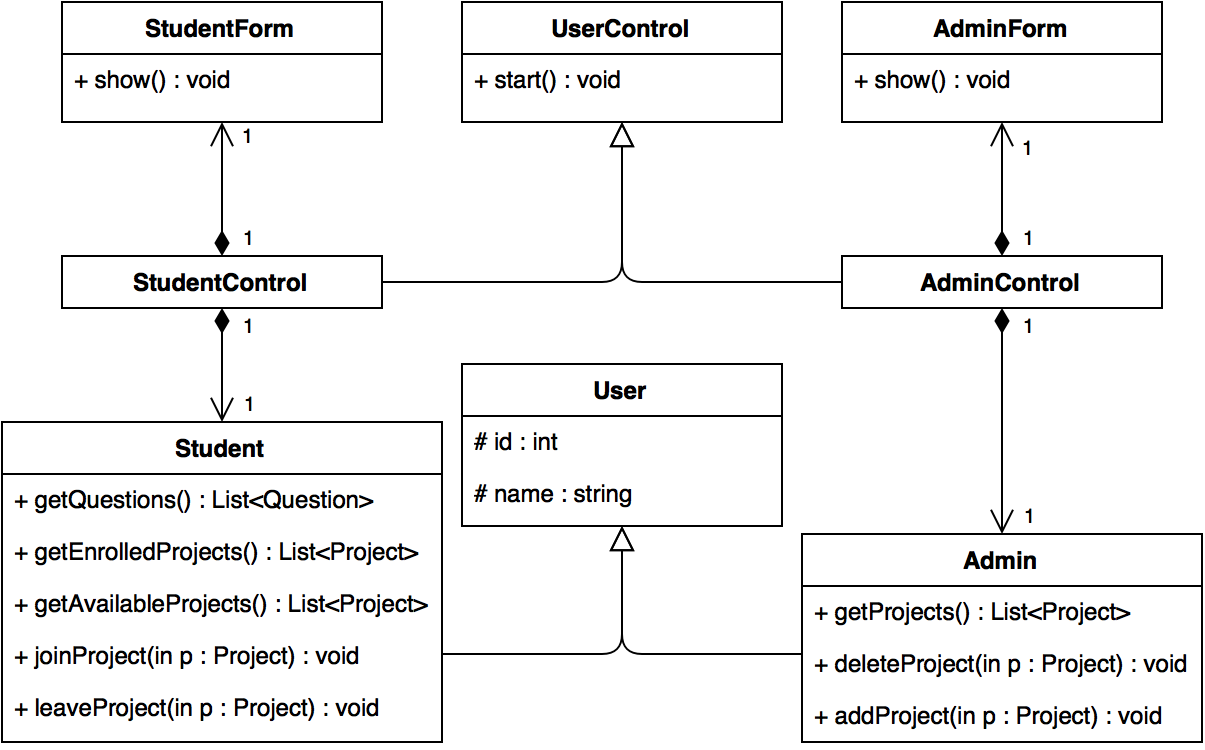
\includegraphics[scale=0.33]{imgs/d3/interfaces/user-options.png}
	\caption{UserOptionsService Class Diagram (\ssref{user-options})}
	\figurelabel{user-options-class-diagram}
\end{figure}

The following table, \tableref{user-ctrl}, gives a detailed breakdown of the UserControl class. Included in the breakdown are the attributes, operations, and any traceability with operations, services, or subsystems.

\begin{table}[H]
    \caption{UserControl Class (\cdref{user-ctrl})} \tablelabel{user-ctrl}
	\begin{tabu} to \textwidth {>{\it}l X}
		\toprule
		Class Identifier & \cdref{user-ctrl} \\
		Name & {\bf UserControl} \\
		Attributes &\\

		Operations &
		\begin{minipage}[t]{\linewidth}
			\begin{itemize}
			    \item {\it public} : start() : return {\bf void}
	        \end{itemize}
	    \end{minipage} \\
	    	Traceability & \ssref{user-options}, \opref{user-ctrl-start}, \sdref{user}\\
		\toprule
	\end{tabu}
\end{table}

The following table, \tableref{student-ctrl}, gives a detailed breakdown of the StudentControl class. Included in the breakdown are the attributes, operations, and any traceability with operations, services, or subsystems.

\begin{table}[H]
    \caption{StudentControl Class (\cdref{student-ctrl})} \tablelabel{student-ctrl}
	\begin{tabu} to \textwidth {>{\it}l X}
		\toprule
		Class Identifier & \cdref{student-ctrl} \\
		Name & {\bf StudentControl} \\
		Attributes & \\

		Operations &
		\begin{minipage}[t]{\linewidth}
			\begin{itemize}
			    \item {\it public} : start() : return {\bf void}
	        \end{itemize}
	    \end{minipage} \\
	    	Traceability & \ssref{user-options}, \sdref{user}\\
		\toprule
	\end{tabu}
\end{table}

The following table, \tableref{admin-ctrl}, gives a detailed breakdown of the AdminControl class. Included in the breakdown are the attributes, operations, and any traceability with operations, services, or subsystems.

\begin{table}[H]
    \caption{AdminControl Class (\cdref{admin-ctrl})} \tablelabel{admin-ctrl}
	\begin{tabu} to \textwidth {>{\it}l X}
		\toprule
		Class Identifier & \cdref{admin-ctrl} \\
		Name & {\bf AdminControl} \\
		Attributes & \\

		Operations &
		\begin{minipage}[t]{\linewidth}
			\begin{itemize}
			    \item {\it public} : start() : return {\bf void}
	        \end{itemize}
	    \end{minipage} \\
	    	Traceability & \ssref{user-options}, \sdref{user}\\
		\toprule
	\end{tabu}
\end{table}

The following table, \tableref{student-form}, gives a detailed breakdown of the StudentForm class. Included in the breakdown are the attributes, operations, and any traceability with operations, services, or subsystems.

\begin{table}[H]
    \caption{StudentForm Class (\cdref{student-form})} \tablelabel{student-form}
	\begin{tabu} to \textwidth {>{\it}l X}
		\toprule
		Class Identifier & \cdref{student-form} \\
		Name & {\bf StudentForm} \\
		Attributes & \\

		Operations &
		\begin{minipage}[t]{\linewidth}
			\begin{itemize}
			    \item {\it public} : show(\underline{in} available : {\bf List<Project>}, \underline{in} enrolled : {\bf List<Project>}) : return {\bf void}
	        \end{itemize}
	    \end{minipage} \\
	    	Traceability & \ssref{user-options}, \sdref{user} \\
		\toprule
	\end{tabu}
\end{table}

The following table, \tableref{admin-form}, gives a detailed breakdown of the AdminForm class. Included in the breakdown are the attributes, operations, and any traceability with operations, services, or subsystems.

\begin{table}[H]
    \caption{AdminForm Class (\cdref{admin-form})} \tablelabel{admin-form}
	\begin{tabu} to \textwidth {>{\it}l X}
		\toprule
		Class Identifier & \cdref{admin-form} \\
		Name & {\bf AdminForm} \\
		Attributes & \\

		Operations &
		\begin{minipage}[t]{\linewidth}
			\begin{itemize}
			    \item {\it public} : show(\underline{in} p : {\bf List<Project>}) : return {\bf void}
	        \end{itemize}
	    \end{minipage} \\
	    	Traceability & \ssref{user-options}, \sdref{user}\\
		\toprule
	\end{tabu}
\end{table}

\subsection{ProfileOptionsService (\ssref{profile-options})}

The following table, \tableref{profile-option-classes}, describes each of the classes involved in the ProfileOptionsService service (\ssref{profile-options}) as well as provide a unique indentifier for each.

\begin{table}[H]
	\caption{ProfileOptionsService Classes (\ssref{profile-options})} \tablelabel{profile-option-classes}
	\begin{tabu} to \textwidth {l >{\it}l X}
	    \tableheader{}ID & Class Name & Description \\
		\cdlabel{profile-form}\cdref{profile-form} & ProfileForm & The ProfileForm class is a UI-based class - the only operation that this class has is show. This class displays the information concerning the particular Student User that is currently logged in's Profile.\\
		\cdlabel{profile-ctrl}\cdref{profile-ctrl} & ProfileControl & The ProfileControl class contains only a single operation - start. The ProfileControl class is the control object that controls the displaying and editing of a Student's profile. \\
	\end{tabu}
\end{table}

The following figure, \figureref{profile-options-class-diagram}, is a UML Class Diagram for the classes involved in the ProfileOptionsService service (\ssref{profile-options}).

\begin{figure}[H]
	\centering{}
	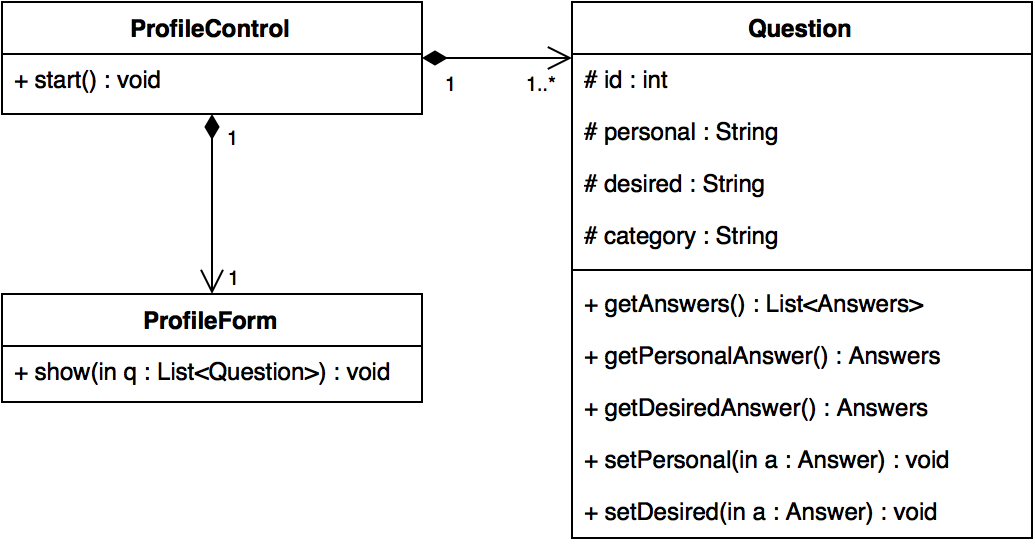
\includegraphics[scale=0.33]{imgs/d3/interfaces/profile-options.png}
	\caption{ProfileOptionsService Class Diagram (\ssref{profile-options})}
	\figurelabel{profile-options-class-diagram}
\end{figure}

The following table, \tableref{profile-form}, gives a detailed breakdown of the ProfileForm class. Included in the breakdown are the attributes, operations, and any traceability with operations, services, or subsystems.

\begin{table}[H]
    \caption{ProfileForm Class (\cdref{profile-form})} \tablelabel{profile-form}
	\begin{tabu} to \textwidth {>{\it}l X}
		\toprule
		Class Identifier & \cdref{profile-form} \\
		Name & {\bf ProfileForm} \\
		Attributes & \\

		Operations &
		\begin{minipage}[t]{\linewidth}
			\begin{itemize}
			    \item {\it public} : show(\underline{in} q : {\bf List<Question>}) : return {\bf void}
	        \end{itemize}
	    \end{minipage} \\
	    	Traceability & \ssref{profile-options}, \sdref{profile}\\
		\toprule
	\end{tabu}
\end{table}

The following table, \tableref{profile-ctrl}, gives a detailed breakdown of the ProfileControl class. Included in the breakdown are the attributes, operations, and any traceability with operations, services, or subsystems.

\begin{table}[H]
    \caption{ProfileControl Class (\cdref{profile-ctrl})} \tablelabel{profile-ctrl}
	\begin{tabu} to \textwidth {>{\it}l X}
		\toprule
		Class Identifier & \cdref{profile-ctrl} \\
		Name & {\bf ProfileControl} \\
		Attributes & \\

		Operations &
		\begin{minipage}[t]{\linewidth}
			\begin{itemize}
			    \item {\it public} : start() : return {\bf void}
	        \end{itemize}
	    \end{minipage} \\
	    	Traceability & \ssref{profile-options}, \opref{profile-ctrl-start}, \sdref{profile}\\
		\toprule
	\end{tabu}
\end{table}

\subsection{ProjectOptionsService (\ssref{project-options})}

The following table, \tableref{project-option-classes}, describes each of the classes involved in the ProjectOptionsService service (\ssref{project-options}) as well as provide a unique indentifier for each.

\begin{table}[H]
	\caption{ProjectOptionsService Classes (\ssref{project-options})} \tablelabel{project-option-classes}
	\begin{tabu} to \textwidth {l >{\it}l X}
	    \tableheader{}ID & Class Name & Description \\
		\cdlabel{project-ctrl}\cdref{project-ctrl} & ProjectControl & The ProjectControl class contains only a single operation - start. The ProjectControl class is the control object that controls the displaying and editing of an Admin's projects.\\
		\cdlabel{project-form}\cdref{project-form} & ProjectForm & The ProjectForm class is a UI-based class - the only operation that this class has is show. This class displays the information concerning the particular Admin User that is currently logged in's Projects.\\
	\end{tabu}
\end{table}

The following figure, \figureref{project-options-class-diagram}, is a UML Class Diagram for the classes involved in the ProjectsOptionsService service (\ssref{project-options}).

\begin{figure}[H]
	\centering{}
	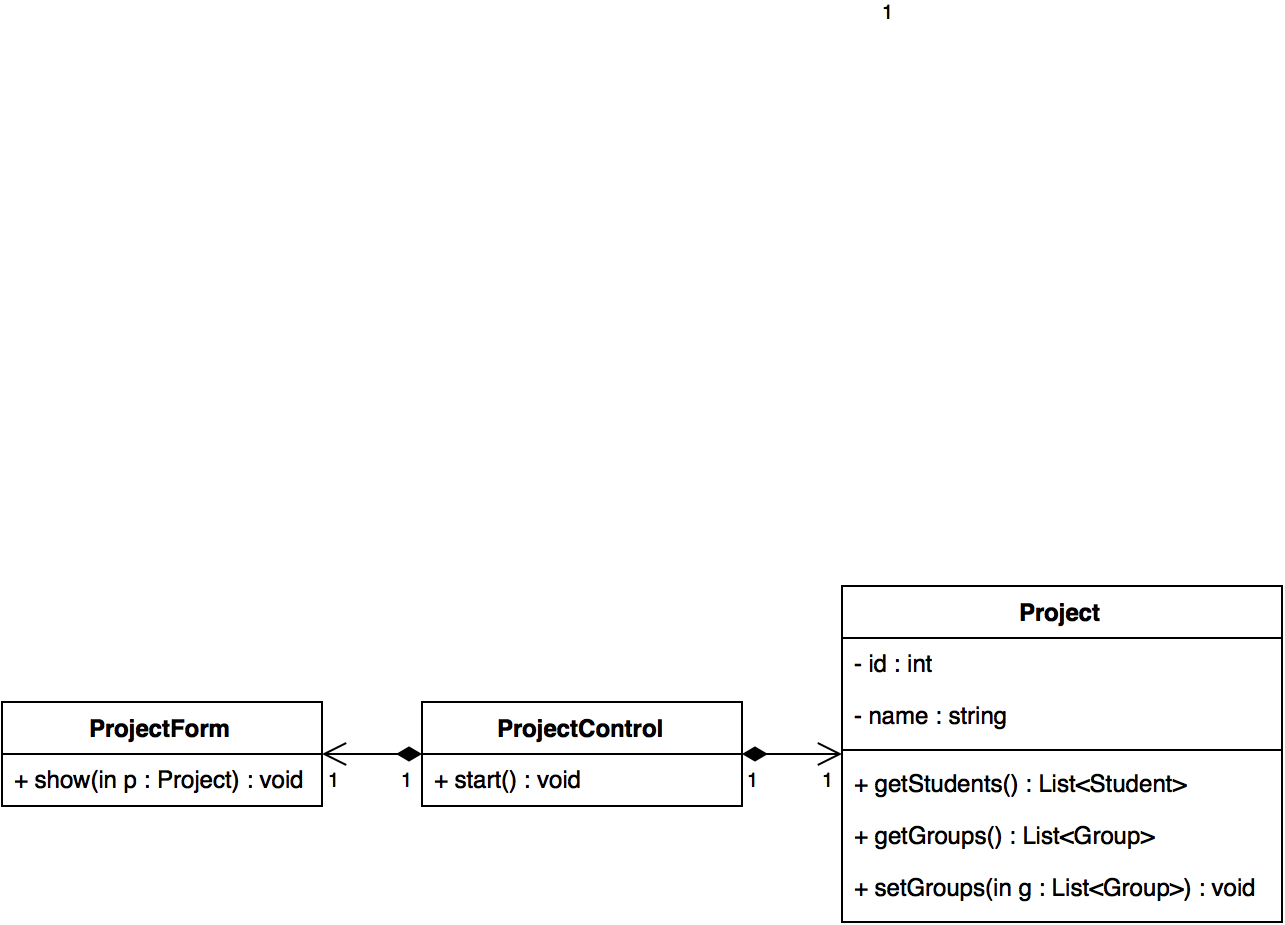
\includegraphics[scale=0.35]{imgs/d3/interfaces/project-options.png}
	\caption{ProjectOptionsService Class Diagram (\ssref{project-options})}
	\figurelabel{project-options-class-diagram}
\end{figure}

The following table, \tableref{project-ctrl}, gives a detailed breakdown of the ProjectControl class. Included in the breakdown are the attributes, operations, and any traceability with operations, services, or subsystems.

\begin{table}[H]
    \caption{ProjectControl Class (\cdref{project-ctrl})} \tablelabel{project-ctrl}
	\begin{tabu} to \textwidth {>{\it}l X}
		\toprule
		Class Identifier & \cdref{project-ctrl} \\
		Name & {\bf ProjectControl} \\
		Attributes & \\

		Operations &
		\begin{minipage}[t]{\linewidth}
			\begin{itemize}
			    \item {\it public} : start() : return {\bf void}
	        \end{itemize}
	    \end{minipage} \\
	    	Traceability & \ssref{project-options}, \opref{project-ctrl-start}, \sdref{project}\\
		\toprule
	\end{tabu}
\end{table}

The following table, \tableref{project-form}, gives a detailed breakdown of the ProjectForm class. Included in the breakdown are the attributes, operations, and any traceability with operations, services, or subsystems.

\begin{table}[H]
    \caption{ProjectForm Class (\cdref{project-form})} \tablelabel{project-form}
	\begin{tabu} to \textwidth {>{\it}l X}
		\toprule
		Class Identifier & \cdref{project-form} \\
		Name & {\bf ProjectForm} \\
		Attributes & \\

		Operations &
		\begin{minipage}[t]{\linewidth}
			\begin{itemize}
			    \item {\it public} : show(\underline{in} p : {\bf Project}) : return {\bf void}
	        \end{itemize}
	    \end{minipage} \\
	    	Traceability & \ssref{project-options}, \sdref{project}\\
		\toprule
	\end{tabu}
\end{table}

\subsection{PPIDOptionsService (\ssref{ppid-options})}

The following table, \tableref{ppid-option-classes}, describes each of the classes involved in the PPIDOptionsService service (\ssref{ppid-options}) as well as provide a unique indentifier for each.

\begin{table}[H]
	\caption{PPIDOptionsService Classes (\ssref{ppid-options})} \tablelabel{ppid-option-classes}
	\begin{tabu} to \textwidth {l >{\it}l X}
	    \tableheader{}ID & Class Name & Description \\
		\cdlabel{grouper}\cdref{grouper} & Grouper & The Grouper class has only a single operation - group. This class is in charge of adding a list of Students into a Group object.\\
		\cdlabel{matcher}\cdref{matcher} & Matcher & The Matcher class has one operation that gets overloaded - match. The overloaded aspect assures that the Matcher can match individual Students to other Students as well as Groups to Students.\\
		\cdlabel{split-smallest}\cdref{split-smallest} & SplitSmallest & The SplitSmallest class inherits from the Grouper class and simply splits the smallest Group into a list of individual Students.\\
		\cdlabel{percent-distance}\cdref{percent-distance} & PercentDistance & The PercentDistance class inherits from the Matcher class and simply returns the match percent of either two Students or a Student and a Group.\\
		\cdlabel{ppid-ctrl}\cdref{ppid-ctrl} & PPIDControl & The PPIDControl class contains only a single operation - start. The PPIDControl class is the control object responsible for handling the running of the PPID algorithm.\\
		\cdlabel{ppid-form}\cdref{ppid-form} & PPIDForm & The PPIDForm class is a UI-based class - the only operation that this class has is show. This class displays the information concerning the last run PPID algorithm for a specific Project.\\
	\end{tabu}
\end{table}

The following figure, \figureref{ppid-options-class-diagram}, is a UML Class Diagram for the classes involved in the PPIDOptionsService service (\ssref{ppid-options}).

\begin{figure}[H]
	\centering{}
	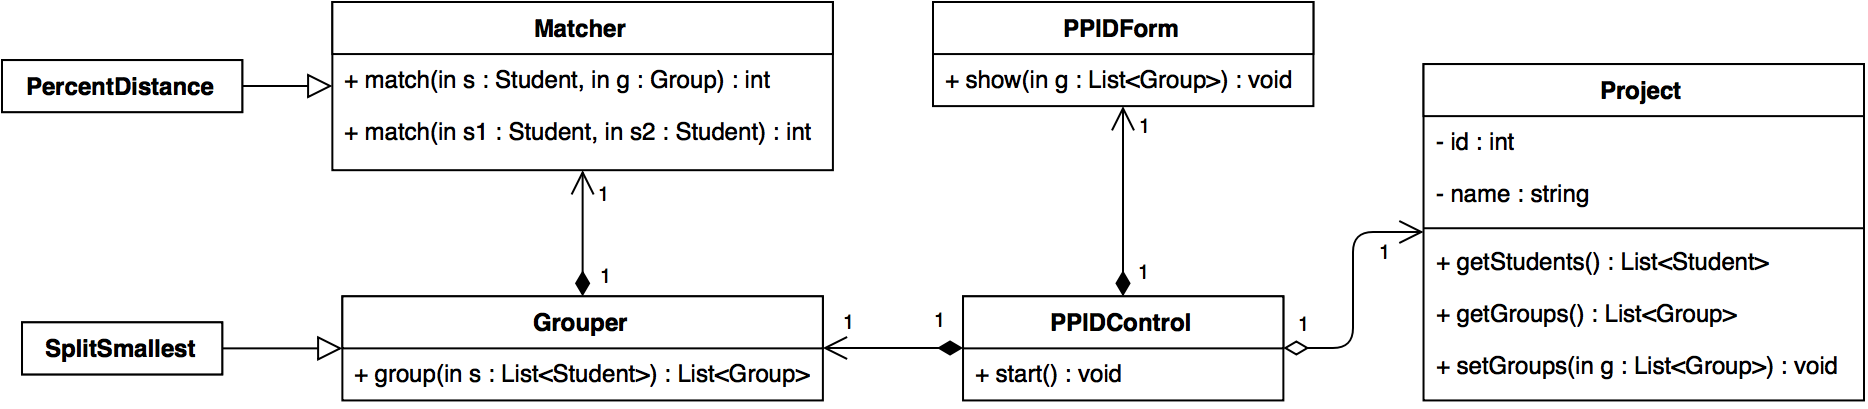
\includegraphics[scale=0.27]{imgs/d3/interfaces/ppid-options.png}
	\caption{PPIDOptionsService Class Diagram (\ssref{ppid-options})}
	\figurelabel{ppid-options-class-diagram}
\end{figure}

The following table, \tableref{grouper}, gives a detailed breakdown of the Grouper class. Included in the breakdown are the attributes, operations, and any traceability with operations, services, or subsystems.

\begin{table}[H]
    \caption{Grouper Class (\cdref{grouper})} \tablelabel{grouper}
	\begin{tabu} to \textwidth {>{\it}l X}
		\toprule
		Class Identifier & \cdref{grouper} \\
		Name & {\bf Grouper} \\
		Attributes & \\

		Operations &
		\begin{minipage}[t]{\linewidth}
			\begin{itemize}
			    \item {\it public} : group(\underline{in} s : {\bf List<Student>}) : return {\bf List<Group>}
	        \end{itemize}
	    \end{minipage} \\
	    	Traceability & \ssref{ppid-options}, \sdref{ppid}\\
		\toprule
	\end{tabu}
\end{table}

The following table, \tableref{matcher}, gives a detailed breakdown of the Matcher class. Included in the breakdown are the attributes, operations, and any traceability with operations, services, or subsystems.

\begin{table}[H]
    \caption{Matcher Class (\cdref{matcher})} \tablelabel{matcher}
	\begin{tabu} to \textwidth {>{\it}l X}
		\toprule
		Class Identifier & \cdref{matcher} \\
		Name & {\bf Matcher} \\
		Attributes & \\

		Operations &
		\begin{minipage}[t]{\linewidth}
			\begin{itemize}
			    \item {\it public} : match(\underline{in} s : {\bf Student}, \underline{in} g : {\bf Group}) : return {\bf int}
			    \item {\it public} : match(\underline{in} s1 : {\bf Student}, \underline{in} s2 : {\bf Student}) : return {\bf int}
	        \end{itemize}
	    \end{minipage} \\
	    	Traceability & \ssref{ppid-options}, \sdref{ppid}\\
		\toprule
	\end{tabu}
\end{table}

The following table, \tableref{split-smallest}, gives a detailed breakdown of the SplitSmallest class. Included in the breakdown are the attributes, operations, and any traceability with operations, services, or subsystems.

\begin{table}[H]
    \caption{SplitSmallest Class (\cdref{split-smallest})} \tablelabel{split-smallest}
	\begin{tabu} to \textwidth {>{\it}l X}
		\toprule
		Class Identifier & \cdref{split-smallest} \\
		Name & {\bf SplitSmallest} \\
		Attributes & \\

		Operations &
		\begin{minipage}[t]{\linewidth}
			\begin{itemize}
			    \item {\it public} : match(\underline{in} s : {\bf Student}, \underline{in} g : {\bf Group}) : return {\bf int}
			    \item {\it public} : match(\underline{in} s1 : {\bf Student}, \underline{in} s2 : {\bf Student}) : return {\bf int}
	        \end{itemize}
	    \end{minipage} \\
	    	Traceability & \ssref{ppid-options}, \sdref{ppid}\\
		\toprule
	\end{tabu}
\end{table}

The following table, \tableref{percent-distance}, gives a detailed breakdown of the PercentDistance class. Included in the breakdown are the attributes, operations, and any traceability with operations, services, or subsystems.

\begin{table}[H]
    \caption{PercentDistance Class (\cdref{percent-distance})} \tablelabel{percent-distance}
	\begin{tabu} to \textwidth {>{\it}l X}
		\toprule
		Class Identifier & \cdref{percent-distance} \\
		Name & {\bf PercentDistance} \\
		Attributes & \\

		Operations &
		\begin{minipage}[t]{\linewidth}
			\begin{itemize}
			    \item {\it public} : group(\underline{in} s : {\bf List<Student>}) : return {\bf List<Group>}
	        \end{itemize}
	    \end{minipage} \\
	    	Traceability & \ssref{ppid-options}, \sdref{ppid}\\
		\toprule
	\end{tabu}
\end{table}

The following table, \tableref{ppid-ctrl}, gives a detailed breakdown of the PPIDControl class. Included in the breakdown are the attributes, operations, and any traceability with operations, services, or subsystems.

\begin{table}[H]
    \caption{PPIDControl Class (\cdref{ppid-ctrl})} \tablelabel{ppid-ctrl}
	\begin{tabu} to \textwidth {>{\it}l X}
		\toprule
		Class Identifier & \cdref{ppid-ctrl} \\
		Name & {\bf PPIDControl} \\
		Attributes & \\

		Operations &
		\begin{minipage}[t]{\linewidth}
			\begin{itemize}
			    \item {\it public} : start() : return {\bf void}
	        \end{itemize}
	    \end{minipage} \\
	    	Traceability & \ssref{ppid-options}, \opref{ppid-ctrl-start}, \sdref{ppid}\\
		\toprule
	\end{tabu}
\end{table}

The following table, \tableref{ppid-form}, gives a detailed breakdown of the PPIDForm class. Included in the breakdown are the attributes, operations, and any traceability with operations, services, or subsystems.

\begin{table}[H]
    \caption{PPIDForm Class (\cdref{ppid-form})} \tablelabel{ppid-form}
	\begin{tabu} to \textwidth {>{\it}l X}
		\toprule
		Class Identifier & \cdref{ppid-form} \\
		Name & {\bf PPIDForm} \\
		Attributes & \\

		Operations &
		\begin{minipage}[t]{\linewidth}
			\begin{itemize}
			    \item {\it public} : show(\underline{in} g : {\bf List<Group>}) : return {\bf void}
	        \end{itemize}
	    \end{minipage} \\
	    	Traceability & \ssref{ppid-options}, \sdref{ppid}\\
		\toprule
	\end{tabu}
\end{table}

\subsection{UserService (\ssref{user})}

The following table, \tableref{user-classes}, describes each of the classes involved in the UserService service (\ssref{user}) as well as provide a unique indentifier for each.

\begin{table}[H]
	\caption{UserService Classes (\ssref{user})} \tablelabel{user-classes}
	\begin{tabu} to \textwidth {l >{\it}l X}
	    \tableheader{}ID & Class Name & Description \\
        \cdlabel{user-storage}\cdref{user-storage} & UserStorage & The UserStorage class offers two operations - getStudent and getAdmin. This class simply returns either a Student object or an Admin object.\\
	\end{tabu}
\end{table}

The following figure, \figureref{user-class-diagram}, is a UML Class Diagram for the classes involved in the UserService service (\ssref{user}).

\begin{figure}[H]
	\centering{}
	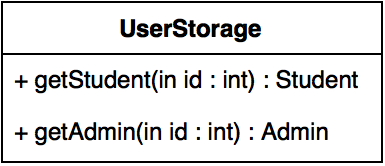
\includegraphics[scale=0.35]{imgs/d3/interfaces/user.png}
	\caption{UserService Class Diagram (\ssref{user})}
	\figurelabel{user-class-diagram}
\end{figure}

The following table, \tableref{userstorage}, gives a detailed breakdown of the UserStorage class. Included in the breakdown are the attributes, operations, and any traceability with operations, services, or subsystems.

\begin{table}[H]
    \caption{UserStorage Class (\cdref{user-storage})} \tablelabel{userstorage}
	\begin{tabu} to \textwidth {>{\it}l X}
		\toprule
		Class Identifier & \cdref{user-storage} \\
		Name & {\bf UserStorage} \\
		Attributes & \\

		Operations &
		\begin{minipage}[t]{\linewidth}
			\begin{itemize}
			    \item {\it public} : getStudent(\underline{in} id : {\bf int}) : return {\bf Student}
			    \item {\it public} : getAdmin(\underline{in} id : {\bf int}) : return {\bf Admin}
	        \end{itemize}
	    \end{minipage} \\
	    	Traceability & \ssref{user}, \opref{user-storage-get-student}, \opref{user-storage-get-admin}, \sdref{storage}\\
		\toprule
	\end{tabu}
\end{table}

\subsection{StudentService (\ssref{student})}

The following table, \tableref{student-classes}, describes each of the classes involved in the StudentService service (\ssref{student}) as well as provide a unique indentifier for each.

\begin{table}[H]
	\caption{StudentService Classes (\ssref{student})} \tablelabel{student-classes}
	\begin{tabu} to \textwidth {l >{\it}l X}
	    \tableheader{}ID & Class Name & Description \\
		\cdlabel{student}\cdref{student} & Student & The Student class contains several attributes: a unique ID, a name, both inherited from the User class, a collection of responses, and their join-status with regards to projects. Their methods revolve around the handling of their profiles, such as modifying response values. This class inherits from the User class. \\
		\cdlabel{realstudent}\cdref{realstudent} & RealStudent & The RealStudent class inherits from the Student class and contains the actual information pulled from the StudentStorage object. It is relatively hidden from the rest of the system, though the data can be accessed through the ProxyStudent object.\\
		\cdlabel{proxystudent}\cdref{proxystudent} & ProxyStudent & The ProxyStudent class also inherits from the Student class and provides a proxy or interface to the RealStudent object for the rest of the system. The idea here is to promote `lazy' loading with regards to the information stored in the RealStudent object.\\
		\cdlabel{studentstorage}\cdref{studentstorage} & StudentStorage & The StudentStorage class is a class that provides a set of methods to pull/push data related to the Student user from/to the relational database. The RealStudent object is the only object that directly interacts with this object.\\
	\end{tabu}
\end{table}

The following figure, \figureref{student-class-diagram}, is a UML Class Diagram for the classes involved in the StudentService service (\ssref{student}).

\begin{figure}[H]
	\centering{}
	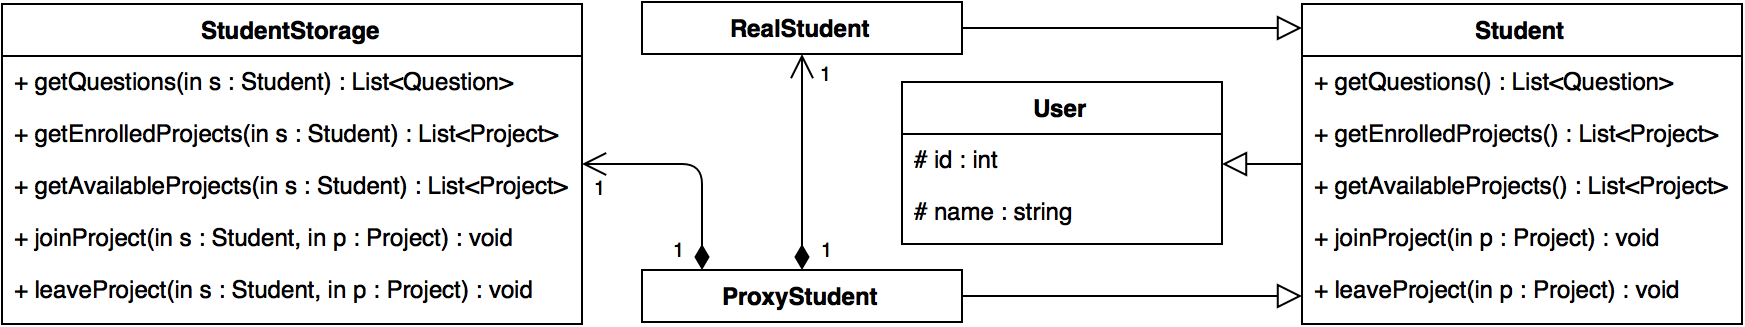
\includegraphics[scale=0.33]{imgs/d3/interfaces/student.png}
	\caption{StudentService Class Diagram (\ssref{student})}
	\figurelabel{student-class-diagram}
\end{figure}

The following table, \tableref{student}, gives a detailed breakdown of the Student class. Included in the breakdown are the attributes, operations, and any traceability with operations, services, or subsystems.

\begin{table}[H]
    \caption{Student Class (\cdref{student})} \tablelabel{student}
	\begin{tabu} to \textwidth {>{\it}l X}
		\toprule
		Class Identifier & \cdref{student} \\
		Name & {\bf Student} \\
		Attributes & 
		\begin{minipage}[t]{\linewidth}
		    \begin{itemize}
		        \item \textit{protected} : ID : {\bf int}
		        \item \textit{protected} : Name: {\bf string}
			\end{itemize}
	    \end{minipage} \\

		Operations &
		\begin{minipage}[t]{\linewidth}
			\begin{itemize}
			    \item {\it public} : getQuestions() : return {\bf List<Question>}
			    \item {\it public} : getEnrolledProjects() : return {\bf List<Project>}
			    \item {\it public} : getAvailableProjects() : return {\bf List<Project>}
			    \item {\it public} : joinProject(\underline{in} p : {\bf Project}) : return {\bf void}
			    \item {\it public} : leaveProject(\underline{in} p : {\bf Project}) : return {\bf void}
	        \end{itemize}
	    \end{minipage} \\
	    	Traceability & \ssref{student}, \opref{user-get-questions}, \opref{user-get-enrolled-projects}, \opref{user-get-available-projects}, \opref{user-join-project}, \opref{user-leave-project}, \sdref{storage}\\
		\toprule
	\end{tabu}
\end{table}

The following table, \tableref{realstudent}, gives a detailed breakdown of the RealStudent class. Included in the breakdown are the attributes, operations, and any traceability with operations, services, or subsystems.

\begin{table}[H]
    \caption{RealStudent Class (\cdref{realstudent})} \tablelabel{realstudent}
	\begin{tabu} to \textwidth {>{\it}l X}
		\toprule
		Class Identifier & \cdref{realstudent} \\
		Name & {\bf RealStudent} \\
		Attributes & 
		\begin{minipage}[t]{\linewidth}
		    \begin{itemize}
		        \item \textit{protected} : ID : {\bf int}
		        \item \textit{protected} : Name: {\bf string}
			\end{itemize}
	    \end{minipage} \\

		Operations &
		\begin{minipage}[t]{\linewidth}
			\begin{itemize}
			    \item {\it public} : getQuestions() : return {\bf List<Question>}
			    \item {\it public} : getEnrolledProjects() : return {\bf List<Project>}
			    \item {\it public} : getAvailableProjects() : return {\bf List<Project>}
			    \item {\it public} : joinProject(\underline{in} p : {\bf Project}) : return {\bf void}
			    \item {\it public} : leaveProject(\underline{in} p : {\bf Project}) : return {\bf void}
	        \end{itemize}
	    \end{minipage} \\
	    	Traceability & \ssref{student}, \sdref{storage}\\
		\toprule
	\end{tabu}
\end{table}

The following table, \tableref{proxystudent}, gives a detailed breakdown of the ProxyStudent class. Included in the breakdown are the attributes, operations, and any traceability with operations, services, or subsystems.

\begin{table}[H]
    \caption{ProxyStudent Class (\cdref{proxystudent})} \tablelabel{proxystudent}
	\begin{tabu} to \textwidth {>{\it}l X}
		\toprule
		Class Identifier & \cdref{proxystudent} \\
		Name & {\bf ProxyStudent} \\
		Attributes & 
		\begin{minipage}[t]{\linewidth}
		    \begin{itemize}
		        \item \textit{protected} : ID : {\bf int}
		        \item \textit{protected} : Name: {\bf string}
			\end{itemize}
	    \end{minipage} \\

		Operations &
		\begin{minipage}[t]{\linewidth}
			\begin{itemize}
			    \item {\it public} : getQuestions() : return {\bf List<Question>}
			    \item {\it public} : getEnrolledProjects() : return {\bf List<Project>}
			    \item {\it public} : getAvailableProjects() : return {\bf List<Project>}
			    \item {\it public} : joinProject(\underline{in} p : {\bf Project}) : return {\bf void}
			    \item {\it public} : leaveProject(\underline{in} p : {\bf Project}) : return {\bf void}
	        \end{itemize}
	    \end{minipage} \\
	    	Traceability & \ssref{student}, \sdref{storage}\\
		\toprule
	\end{tabu}
\end{table}

The following table, \tableref{studentstorage}, gives a detailed breakdown of the StudentStorage class. Included in the breakdown are the attributes, operations, and any traceability with operations, services, or subsystems.

\begin{table}[H]
    \caption{StudentStorage Class (\cdref{studentstorage})} \tablelabel{studentstorage}
	\begin{tabu} to \textwidth {>{\it}l X}
		\toprule
		Class Identifier & \cdref{studentstorage} \\
		Name & {\bf StudentStorage} \\
		Attributes & \\

		Operations &
		\begin{minipage}[t]{\linewidth}
			\begin{itemize}
			    \item {\it public} : getQuestions(\underline{in} s : {\bf Student}) : return {\bf List<Question>}
			    \item {\it public} : getEnrolledProjects(\underline{in} s : {\bf Student}) : return {\bf List<Project>}
			    \item {\it public} : getAvailableProjects(\underline{in} s : {\bf Student}) : return {\bf List<Project>}
			    \item {\it public} : joinProject(\underline{in} s : {\bf Student}, \underline{in} p : {\bf Project}) : return {\bf void}
			    \item {\it public} : leaveProject(\underline{in} s : {\bf Student}, \underline{in} p : {\bf Project}) : return {\bf void}
	        \end{itemize}
	    \end{minipage} \\
	    	Traceability & \ssref{student}, \sdref{storage}\\
		\toprule
	\end{tabu}
\end{table}

\subsection{AdminService (\ssref{admin})}

The following table, \tableref{admin-classes}, describes each of the classes involved in the AdminService service (\ssref{admin}) as well as provide a unique indentifier for each.

\begin{table}[H]
	\caption{AdminService Classes (\ssref{admin})} \tablelabel{admin-classes}
	\begin{tabu} to \textwidth {l >{\it}l X}
	    \tableheader{}ID & Class Name & Description \\
		\cdlabel{admin}\cdref{admin} & Admin & The Admin class contains two attributes - the unique ID, and a name, both inherited from the User class - and several methods revolving around the handling of Project objects. This class inherits from the User class. \\
		\cdlabel{realadmin}\cdref{realadmin} & RealAdmin & The RealAdmin class inherits from the Admin class and contains the actual information pulled from the AdminStorage object. It is relatively hidden from the rest of the system, though the data contained can only be accessed through the ProxyAdmin object. \\
		\cdlabel{proxyadmin}\cdref{proxyadmin} & ProxyAdmin & The ProxyAdmin class also inherits from the Admin class and provides a proxy or interface to the RealAdmin object for the rest of the system. The idea here is to promote `lazy' loading with regards to the information stored in the RealAdmin object.\\
		\cdlabel{adminstorage}\cdref{adminstorage} & AdminStorage & The AdminStorage class is a class that provides a set of methods to pull/push data related to the Admin user from/to the relational database. The RealAdmin object is the only object that directly interacts with this object.\\
	\end{tabu}
\end{table}

The following figure, \figureref{admin-class-diagram}, is a UML Class Diagram for the classes involved in the AdminService service (\ssref{admin}).

\begin{figure}[H]
	\centering{}
	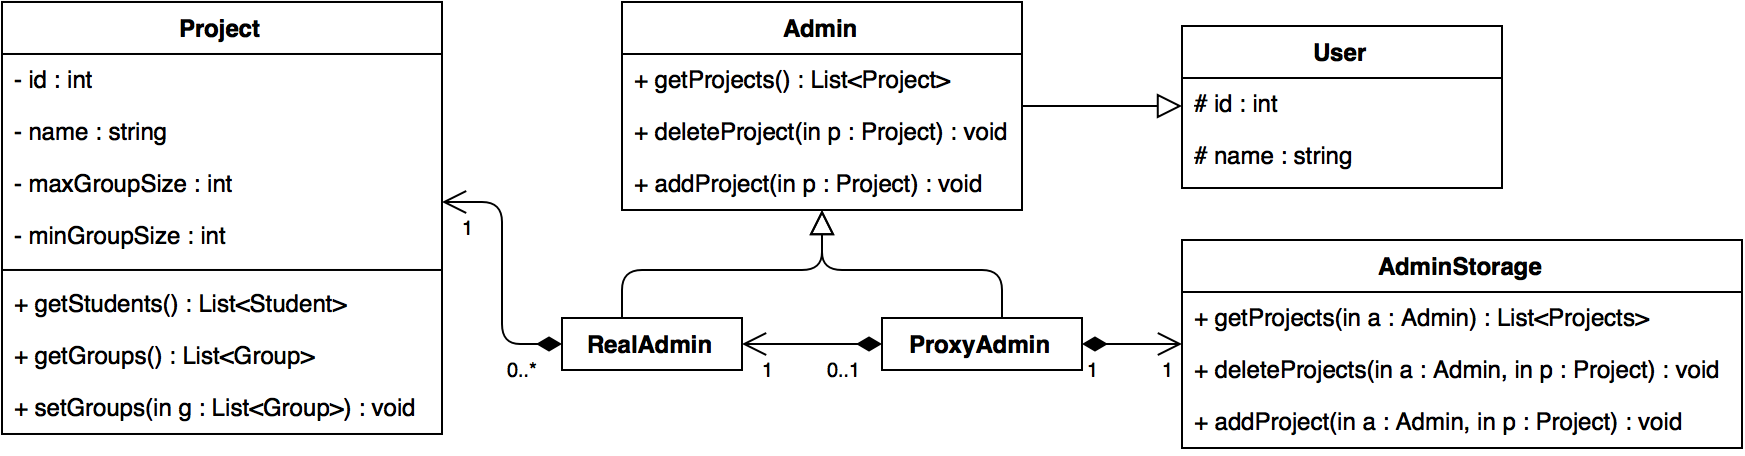
\includegraphics[scale=0.27]{imgs/d3/interfaces/admin.png}
	\caption{AdminService Class Diagram (\ssref{admin})}
	\figurelabel{admin-class-diagram}
\end{figure}

The following table, \tableref{admin}, gives a detailed breakdown of the Admin class. Included in the breakdown are the attributes, operations, and any traceability with operations, services, or subsystems.

\begin{table}[H]
    \caption{Admin Class (\cdref{admin})} \tablelabel{admin}
	\begin{tabu} to \textwidth {>{\it}l X}
		\toprule
		Class Identifier & \cdref{admin} \\
		Name & {\bf Admin} \\
		Attributes & 
		\begin{minipage}[t]{\linewidth}
		    \begin{itemize}
		        \item \textit{protected} : ID : {\bf int}
		        \item \textit{protected} : Name: {\bf string}
			\end{itemize}
	    \end{minipage} \\

		Operations &
		\begin{minipage}[t]{\linewidth}
			\begin{itemize}
			    \item {\it public} : getProjects() : return {\bf List<Project>}
			    \item {\it public} : deleteProject(\underline{in} p : {\bf Project}) : return {\bf void}
			    \item {\it public} : addProject(\underline{in} p : {\bf Project}) : return {\bf void}
	        \end{itemize}
	    \end{minipage} \\
	    	Traceability & \ssref{admin}, \opref{admin-get-projects}, \opref{admin-delete-project}, \opref{admin-add-project}, \sdref{storage}\\
		\toprule
	\end{tabu}
\end{table}

The following table, \tableref{realadmin}, gives a detailed breakdown of the RealAdmin class. Included in the breakdown are the attributes, operations, and any traceability with operations, services, or subsystems.

\begin{table}[H]
    \caption{RealAdmin Class (\cdref{realadmin})} \tablelabel{realadmin}
	\begin{tabu} to \textwidth {>{\it}l X}
		\toprule
		Class Identifier & \cdref{realadmin} \\
		Name & {\bf RealAdmin} \\
		Attributes & 
		\begin{minipage}[t]{\linewidth}
		    \begin{itemize}
		        \item \textit{protected} : ID : {\bf int}
		        \item \textit{protected} : Name: {\bf string}
			\end{itemize}
	    \end{minipage} \\

		Operations &
		\begin{minipage}[t]{\linewidth}
			\begin{itemize}
			    \item {\it public} : getProjects() : return {\bf List<Project>}
			    \item {\it public} : deleteProject(\underline{in} p : {\bf Project}) : return {\bf void}
			    \item {\it public} : addProject(\underline{in} p : {\bf Project}) : return {\bf void}
	        \end{itemize}
	    \end{minipage} \\
	    	Traceability & \ssref{admin}, \sdref{storage}\\
		\toprule
	\end{tabu}
\end{table}

The following table, \tableref{proxyadmin}, gives a detailed breakdown of the ProxyAdmin class. Included in the breakdown are the attributes, operations, and any traceability with operations, services, or subsystems.

\begin{table}[H]
    \caption{ProxyAdmin Class (\cdref{proxyadmin})} \tablelabel{proxyadmin}
	\begin{tabu} to \textwidth {>{\it}l X}
		\toprule
		Class Identifier & \cdref{proxyadmin} \\
		Name & {\bf ProxyAdmin} \\
		Attributes & 
		\begin{minipage}[t]{\linewidth}
		    \begin{itemize}
		        \item \textit{protected} : ID : {\bf int}
		        \item \textit{protected} : Name: {\bf string}
			\end{itemize}
	    \end{minipage} \\

		Operations &
		\begin{minipage}[t]{\linewidth}
			\begin{itemize}
			    \item {\it public} : getProjects() : return {\bf List<Project>}
			    \item {\it public} : deleteProject(\underline{in} p : {\bf Project}) : return {\bf void}
			    \item {\it public} : addProject(\underline{in} p : {\bf Project}) : return {\bf void}
	        \end{itemize}
	    \end{minipage} \\
	    	Traceability & \ssref{admin}, \sdref{storage}\\
		\toprule
	\end{tabu}
\end{table}

The following table, \tableref{adminstorage}, gives a detailed breakdown of the AdminStorage class. Included in the breakdown are the attributes, operations, and any traceability with operations, services, or subsystems.

\begin{table}[H]
    \caption{AdminStorage Class (\cdref{adminstorage})} \tablelabel{adminstorage}
	\begin{tabu} to \textwidth {>{\it}l X}
		\toprule
		Class Identifier & \cdref{adminstorage} \\
		Name & {\bf AdminStorage} \\
		Attributes & \\

		Operations &
		\begin{minipage}[t]{\linewidth}
			\begin{itemize}
			    \item {\it public} : getProjects(\underline{in} a : {\bf Admin}) : return {\bf List<Project>}
			    \item {\it public} : deleteProject(\underline{in} a : {\bf Admin}) : return {\bf void}
			    \item {\it public} : addProject(\underline{in} a : {\bf Admin}) : return {\bf void}
	        \end{itemize}
	    \end{minipage} \\
	    	Traceability & \ssref{admin}, \sdref{storage}\\
		\toprule
	\end{tabu}
\end{table}

\subsection{ProjectService (\ssref{project})}

The following table, \tableref{project-classes}, describes each of the classes involved in the ProjectService service (\ssref{project}) as well as provide a unique indentifier for each.

\begin{table}[H]
	\caption{ProjectService Classes (\ssref{project})} \tablelabel{project-classes}
	\begin{tabu} to \textwidth {l >{\it}l X}
	    \tableheader{}ID & Class Name & Description \\
		\cdlabel{project}\cdref{project} & Project & The Project class contains five attributes: a name, a unique ID, a minimum group size, a maximum group size, and a collection of Student objects. Its methods revolve around simply returning the collection of Students.\\
		\cdlabel{realproject}\cdref{realproject} & RealProject & The RealProject class inherits from the Project class and contains the actual information pulled from the ProjectStorage object. It is relatively hidden from the rest of the system, though the data can be accessed through the ProxyProject object.\\
		\cdlabel{proxyproject}\cdref{proxyproject} & ProxyProject & The ProxyProject also inherits from the Project class and provides a proxy or interface to the RealProject object for the rest of the system. The idea here is to promote `lazy' loading with regards to the information stored in the RealProject object.\\
		\cdlabel{projectstorage}\cdref{projectstorage} & ProjectStorage & The ProjectStorage class is a class that provides a set of methods to pull/push data related to Projects from/to the relational database. The RealProject object is the only object that directly interacts with this object.\\
		\cdlabel{group}\cdref{group} & Group & A Group class is a class that has a collection or list of Student objects. Its methods revolve around adding new Students to the Group or removing Students from the Group.\\
	\end{tabu}
\end{table}

\begin{figure}[H]
	\centering{}
	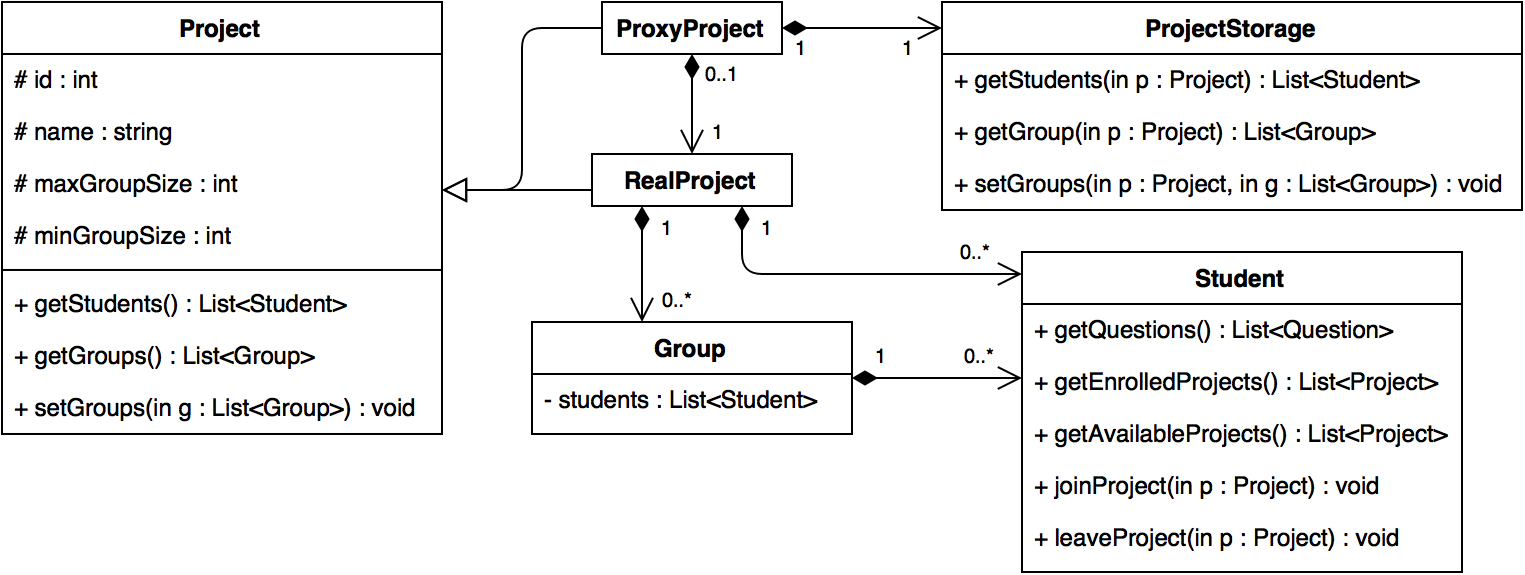
\includegraphics[scale=0.33]{imgs/d3/interfaces/project.png}
	\caption{ProjectService Class Diagram (\ssref{project})}
	\figurelabel{project-class-diagram}
\end{figure}

The following table, \tableref{project}, gives a detailed breakdown of the Project class. Included in the breakdown are the attributes, operations, and any traceability with operations, services, or subsystems.

\begin{table}[H]
    \caption{RealProject Class (\cdref{project})} \tablelabel{project}
	\begin{tabu} to \textwidth {>{\it}l X}
		\toprule
		Class Identifier & \cdref{project} \\
		Name & {\bf RealProject} \\
		Attributes & 
		\begin{minipage}[t]{\linewidth}
		    \begin{itemize}
		        \item \textit{public} : ID : \bf{int}
			\end{itemize}
	    \end{minipage} \\

		Operations &
		\begin{minipage}[t]{\linewidth}
			\begin{enumerate}
			    \item[-] stuff
	        \end{enumerate}
	    \end{minipage} \\
	    	Traceability & \\
		\toprule
	\end{tabu}
\end{table}

The following table, \tableref{realproject}, gives a detailed breakdown of the RealProject class. Included in the breakdown are the attributes, operations, and any traceability with operations, services, or subsystems.

\begin{table}[H]
    \caption{RealProject Class (\cdref{realproject})} \tablelabel{realproject}
	\begin{tabu} to \textwidth {>{\it}l X}
		\toprule
		Class Identifier & \cdref{realproject} \\
		Name & {\bf RealProject} \\
		Attributes & 
		\begin{minipage}[t]{\linewidth}
		    \begin{itemize}
		        \item \textit{public} : ID : \bf{int}
			\end{itemize}
	    \end{minipage} \\

		Operations &
		\begin{minipage}[t]{\linewidth}
			\begin{enumerate}
			    \item[-] stuff
	        \end{enumerate}
	    \end{minipage} \\
	    	Traceability & \\
		\toprule
	\end{tabu}
\end{table}

The following table, \tableref{proxyproject}, gives a detailed breakdown of the ProxyProject class. Included in the breakdown are the attributes, operations, and any traceability with operations, services, or subsystems.

\begin{table}[H]
    \caption{ProxyProject Class (\cdref{proxyproject})} \tablelabel{proxyproject}
	\begin{tabu} to \textwidth {>{\it}l X}
		\toprule
		Class Identifier & \cdref{proxyproject} \\
		Name & {\bf ProxyProject} \\
		Attributes & 
		\begin{minipage}[t]{\linewidth}
		    \begin{itemize}
		        \item \textit{public} : ID : \bf{int}
			\end{itemize}
	    \end{minipage} \\

		Operations &
		\begin{minipage}[t]{\linewidth}
			\begin{enumerate}
			    \item[-] stuff
	        \end{enumerate}
	    \end{minipage} \\
	    	Traceability & \\
		\toprule
	\end{tabu}
\end{table}

The following table, \tableref{projectstorage}, gives a detailed breakdown of the ProjectStorage class. Included in the breakdown are the attributes, operations, and any traceability with operations, services, or subsystems.

\begin{table}[H]
    \caption{ProjectStorage Class (\cdref{projectstorage})} \tablelabel{projectstorage}
	\begin{tabu} to \textwidth {>{\it}l X}
		\toprule
		Class Identifier & \cdref{projectstorage} \\
		Name & {\bf ProjectStorage} \\
		Attributes & 
		\begin{minipage}[t]{\linewidth}
		    \begin{itemize}
		        \item \textit{public} : ID : \bf{int}
			\end{itemize}
	    \end{minipage} \\

		Operations &
		\begin{minipage}[t]{\linewidth}
			\begin{enumerate}
			    \item[-] stuff
	        \end{enumerate}
	    \end{minipage} \\
	    	Traceability & \\
		\toprule
	\end{tabu}
\end{table}

\subsection{QuestionService (\ssref{question})}

The following table, \tableref{question-classes}, describes each of the classes involved in the QuestionService service (\ssref{question}) as well as provide a unique indentifier for each.

\begin{table}[H]
	\caption{QuestionService Classes (\ssref{question})} \tablelabel{question-classes}
	\begin{tabu} to \textwidth {l >{\it}l X}
	    \tableheader{}ID & Class Name & Description \\
		\cdlabel{question}\cdref{question} & Question & The Question class contains four attributes: a String representation of the questions used in the algorithm for the desired and personal versions of the questions, a unique identifier, and the category of the question. \\
		\cdlabel{realquestion}\cdref{realquestion} & RealQuestion & The RealQuestion class inherits from the Question class and contains the actual information pulled from the QuestionStorage object. It is relatively hidden from the rest of the system, though the data can be accessed through the ProxyQuestion object.\\
		\cdlabel{proxyquestion}\cdref{proxyquestion} & ProxyQuestion & The ProxyQuestion also inherits from the Question class and provides a proxy or interface to the RealQuestion object for the rest of the system. The idea here is to promote `lazy' loading with regards to the information stored in the RealQuestion object.\\
		\cdlabel{questionstorage}\cdref{questionstorage} & QuestionStorage & The QuestionStorage class is a class that provides a set of methods to pull/push data related to Questions from/to the relational database. The RealQuestion object is the only object that directly interacts with this object.\\
		\cdlabel{answer}\cdref{answer} & Answer & The Answer class contains three attributes: the question number, a unique identifier, and the set of answers. The methods this class provides revolve around simply returning the required set of answers.\\
	\end{tabu}
\end{table}

\begin{figure}[H]
	\centering{}
	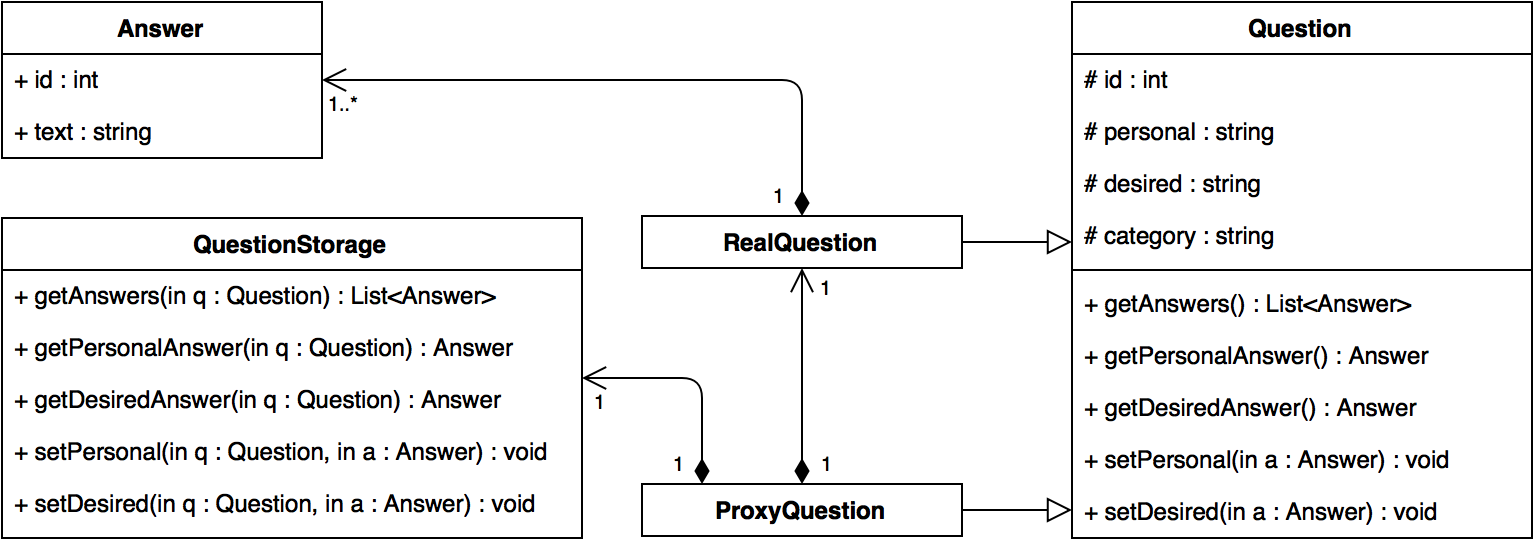
\includegraphics[scale=0.32]{imgs/d3/interfaces/question.png}
	\caption{QuestionService Class Diagram (\ssref{question})}
	\figurelabel{question-class-diagram}
\end{figure}

The following table, \tableref{question}, gives a detailed breakdown of the Question class. Included in the breakdown are the attributes, operations, and any traceability with operations, services, or subsystems.

\begin{table}[H]
    \caption{Question Class (\cdref{question})} \tablelabel{question}
	\begin{tabu} to \textwidth {>{\it}l X}
		\toprule
		Class Identifier & \cdref{question} \\
		Name & {\bf Question} \\
		Attributes & 
		\begin{minipage}[t]{\linewidth}
		    \begin{itemize}
		        \item \textit{public} : ID : \bf{int}
			\end{itemize}
	    \end{minipage} \\

		Operations &
		\begin{minipage}[t]{\linewidth}
			\begin{enumerate}
			    \item[-] stuff
	        \end{enumerate}
	    \end{minipage} \\
	    	Traceability & \\
		\toprule
	\end{tabu}
\end{table}

The following table, \tableref{realquestion}, gives a detailed breakdown of the RealQuestion class. Included in the breakdown are the attributes, operations, and any traceability with operations, services, or subsystems.

\begin{table}[H]
    \caption{RealQuestion Class (\cdref{realquestion})} \tablelabel{realquestion}
	\begin{tabu} to \textwidth {>{\it}l X}
		\toprule
		Class Identifier & \cdref{realquestion} \\
		Name & {\bf RealQuestion} \\
		Attributes & 
		\begin{minipage}[t]{\linewidth}
		    \begin{itemize}
		        \item \textit{public} : ID : \bf{int}
			\end{itemize}
	    \end{minipage} \\

		Operations &
		\begin{minipage}[t]{\linewidth}
			\begin{enumerate}
			    \item[-] stuff
	        \end{enumerate}
	    \end{minipage} \\
	    	Traceability & \\
		\toprule
	\end{tabu}
\end{table}

The following table, \tableref{proxyquestion}, gives a detailed breakdown of the ProxyQuestion class. Included in the breakdown are the attributes, operations, and any traceability with operations, services, or subsystems.

\begin{table}[H]
    \caption{ProxyQuestion Class (\cdref{proxyquestion})} \tablelabel{proxyquestion}
	\begin{tabu} to \textwidth {>{\it}l X}
		\toprule
		Class Identifier & \cdref{proxyquestion} \\
		Name & {\bf ProxyQuestion} \\
		Attributes & 
		\begin{minipage}[t]{\linewidth}
		    \begin{itemize}
		        \item \textit{public} : ID : \bf{int}
			\end{itemize}
	    \end{minipage} \\

		Operations &
		\begin{minipage}[t]{\linewidth}
			\begin{enumerate}
			    \item[-] stuff
	        \end{enumerate}
	    \end{minipage} \\
	    	Traceability & \\
		\toprule
	\end{tabu}
\end{table}

The following table, \tableref{questionstorage}, gives a detailed breakdown of the QuestionStorage class. Included in the breakdown are the attributes, operations, and any traceability with operations, services, or subsystems.

\begin{table}[H]
    \caption{QuestionStorage Class (\cdref{questionstorage})} \tablelabel{questionstorage}
	\begin{tabu} to \textwidth {>{\it}l X}
		\toprule
		Class Identifier & \cdref{questionstorage} \\
		Name & {\bf QuestionStorage} \\
		Attributes & 
		\begin{minipage}[t]{\linewidth}
		    \begin{itemize}
		        \item \textit{public} : ID : \bf{int}
			\end{itemize}
	    \end{minipage} \\

		Operations &
		\begin{minipage}[t]{\linewidth}
			\begin{enumerate}
			    \item[-] stuff
	        \end{enumerate}
	    \end{minipage} \\
	    	Traceability & \\
		\toprule
	\end{tabu}
\end{table}

The following table, \tableref{answer}, gives a detailed breakdown of the Answer class. Included in the breakdown are the attributes, operations, and any traceability with operations, services, or subsystems.

\begin{table}[H]
    \caption{Answer Class (\cdref{answer})} \tablelabel{answer}
	\begin{tabu} to \textwidth {>{\it}l X}
		\toprule
		Class Identifier & \cdref{answer} \\
		Name & {\bf Answer} \\
		Attributes & 
		\begin{minipage}[t]{\linewidth}
		    \begin{itemize}
		        \item \textit{public} : ID : \bf{int}
			\end{itemize}
	    \end{minipage} \\

		Operations &
		\begin{minipage}[t]{\linewidth}
			\begin{enumerate}
			    \item[-] stuff
	        \end{enumerate}
	    \end{minipage} \\
	    	Traceability & \\
		\toprule
	\end{tabu}
\end{table}

The following table, \tableref{group}, gives a detailed breakdown of the Group class. Included in the breakdown are the attributes, operations, and any traceability with operations, services, or subsystems.

\begin{table}[H]
    \caption{Group Class (\cdref{group})} \tablelabel{group}
	\begin{tabu} to \textwidth {>{\it}l X}
		\toprule
		Class Identifier & \cdref{group} \\
		Name & {\bf Group} \\
		Attributes & 
		\begin{minipage}[t]{\linewidth}
		    \begin{itemize}
		        \item \textit{public} : ID : \bf{int}
			\end{itemize}
	    \end{minipage} \\

		Operations &
		\begin{minipage}[t]{\linewidth}
			\begin{enumerate}
			    \item[-] stuff
	        \end{enumerate}
	    \end{minipage} \\
	    	Traceability & \\
		\toprule
	\end{tabu}
\end{table}

\end{document}
